\documentclass[10pt,a4paper]{article}
\usepackage[margin=0.7in]{geometry}
\usepackage[T1]{fontenc}
\usepackage[utf8]{inputenc}
\usepackage{lmodern,amsmath,amssymb,booktabs,array,enumitem}
\usepackage[expansion=false]{microtype}
\usepackage{xurl,hyperref,pdflscape,tabularx,algorithm,algpseudocode,graphicx,tikz}
\hypersetup{hidelinks}
\newcolumntype{Y}{>{\raggedright\arraybackslash}X}
\newcolumntype{L}[1]{>{\raggedright\arraybackslash}p{#1}}
\newcommand{\NA}{\mathrm{N/A}}
\newcommand{\CE}{\operatorname{CE}}
\newcommand{\meas}{\textnormal{[MEASURE]}}
\setlength{\parindent}{0pt}
\setlength{\parskip}{4pt}
\setlength{\tabcolsep}{3pt}
\renewcommand{\arraystretch}{1.12}
\title{\textbf{Computer Networks: Phase 2}\\[5pt]
Poisoning, Retention and Legitimate Adaptation\\
in Federated Continual Intrusion Detection}
\author{Saneedullah (23I-2568) \qquad Ahmed Bilal (23I-2581)}
\date{8 October 2026}
\begin{document}
\maketitle
\begin{abstract}
Federated intrusion detectors must learn emerging attack families while retaining useful discrimination. Poisoned training labels can distort both acquisition and the memory used during subsequent adaptation. Existing studies establish clean federated class-incremental learning, client label-flipping susceptibility and uncertainty-driven memory selection, but provide limited joint evidence on source-specific damage after attacker withdrawal and the acquisition cost of admission defenses. We propose a controlled study using CICIDS2017, with CICIoT2023 as an external check. Five persistent clients train a common 128/64 multilayer perceptron using fine-tuning, EWC-style accumulated importance or DER++. An oblivious source-to-benign labeling intervention affects one client during the second supervised experience. Eligible-source doses, development pilots and paired clean controls determine whether the intervention is informative. We compare class-aware admission with global selection at matched client quotas, using unique-ID reservoir replay. Source recall and clean-matched targeted error test poisoning damage; new-family F1 measures adaptation; previously learned-family scores quantify collateral change. Twelve paired seeds, two declared Holm families, signed-rank tests and symmetry-qualified permutation intervals support analysis. The intended contribution is a reproducible security--adaptation protocol and a falsifiable admission heuristic. This proposal reports a design; experimental outcomes and deployment performance remain to be measured.
\end{abstract}
\noindent\textbf{Keywords:} continual learning; federated IDS; label poisoning; replay memory; legitimate adaptation.

\section{Introduction and Scope}
Attack families change. Learning incoming families can erase earlier discrimination, while replay preserves possibly corrupted examples. A federated detector inherits information from clients with different class support. We study client label corruption, continual memory and admission decisions.

Phase 1 identifies ``Continual Learning for Network Security,'' warns that ``If clustering goes wrong, every later step is affected,'' and records an assumption that ``the coordinating server and all clients are honest.'' Its adaptation-security gap concerns attackers who ``specifically target the adaptation mechanism itself'' \cite{phase1}. Ge et al. investigate staged unknown-DoS discovery, Wu et al. combine federated class acquisition with compressed communication, and Luo et al. address RF authentication drift \cite{ge,wu,luo}. We retain the federated poisoning question, narrow resource evaluation to measured host and transmission costs, and defer drift-detector evasion and RF spoofing. Phase 1 remains unchanged.

Our questions are explicit. \textbf{RQ1:} how do fine-tuning, EWC-style importance and DER++ differ in immediate source-family recall damage and targeted error after poison withdrawal? \textbf{RQ2:} does class-aware admission change those security outcomes and legitimate new-family acquisition compared with equally sized global admission? \textbf{RQ3:} which memory and selection mechanisms explain the observed differences, and what measured computation and communication do they require?

The proposed study will simulate five flow clients and compare source-family damage with legitimate acquisition under matched admission volumes. Phase 2 establishes the literature basis, research gap, experimental protocol and methodology architecture; the reported performance figures belong to the cited studies.

\section{Deliverable 1: Extended Literature Review}
\subsection{Corpus and Selection Criteria}
Seven additional original experimental papers from 2025--2026 have free manuscripts and verified publication records (Table~\ref{tab:corpus}). Older references supply methods only.

Clarivate released the 2025 JCR update on 18 June 2025 \cite{clarivate}. Journal quartiles below refer to the 2024 JIF category edition. Archived rows support these values; primary journal profiles remain unverified. DAC qualifies as peer-reviewed ACM/IEEE proceedings, without a journal quartile.
% VERIFY: confirm the six category-specific journal quartiles in primary Clarivate profiles for the 2025 JCR/2024 JIF edition.

\begin{table}[htbp]
\centering\footnotesize
\caption{Seven-paper corpus. IS means Computer Science, Information Systems; EM means Engineering, Multidisciplinary. Quartiles require the primary-profile check noted above.}
\label{tab:corpus}
\begin{tabularx}{\linewidth}{L{2.5cm}Y L{2.1cm}L{1.9cm}L{2.0cm}}
\toprule
Study & Venue / publisher & Year; access version & Category; quartile; edition & Protocol role\\
\midrule
Carillo et al. \cite{carillo} & IEEE Transactions on Network and Service Management & 2026; author & IS; Q1; JCR 2025 & Clean federated CIL\\
Lavaur et al. \cite{lavaur} & Computers \& Security; Elsevier & 2025; institutional author & IS; Q1; JCR 2025 & Label-flip controls\\
Fuhrman et al. \cite{cnd} & 62nd ACM/IEEE DAC & 2025; arXiv author & Proceedings; quartile $\NA$ & Novelty detection\\
Sameera et al. \cite{wei} & Journal of Information Security and Applications; Elsevier & 2025; arXiv v2 & IS; Q2; JCR 2025 & Server validation gate\\
Cerasuolo et al. \cite{cerasuolo} & Computer Networks; Elsevier & 2025; author & IS; Q1; JCR 2025 & CIL/memory reference\\
Guo et al. \cite{guo} & Future Internet; MDPI & 2025; publisher & IS; Q2; JCR 2025 & Memory selection\\
Prasad et al. \cite{ensemble} & Computer Modeling in Engineering \& Sciences; Tech Science Press & 2026; publisher & EM; Q2; JCR 2025 & Streaming gate comparator\\
\bottomrule
\end{tabularx}
\end{table}

\subsection{Thematic Synthesis}
Table~\ref{tab:taxonomy} classifies all ten studies.

\begin{landscape}
\begin{table}[p]
\centering\footnotesize
\caption{Taxonomy of the seven additions and three Phase 1 sources. CIL means class-incremental learning; FL means federated learning.}
\label{tab:taxonomy}
\begin{tabularx}{\linewidth}{L{2.4cm}Y Y Y Y Y Y}
\toprule
Study & Learning setting & Threat model tested & Defense type & Memory mechanism & Modality & Poisoning with continual learning evidence\\
\midrule
Ge 2026 \cite{ge} & Central unknown-DoS discovery/CIL & Held-out DoS; clean training & AE, HDBSCAN, distillation & Historical knowledge transfer & NSL-KDD flows & Discovery security motivates extension\\
Wu 2026 \cite{wu} & Federated CIL & Honest participants & Head-protected compression & Exemplars/distillation & IoT/IIoT flow vectors & Malicious participants excluded\\
Luo 2026 \cite{luo} & Fixed-device drift adaptation & Synthetic RF drift & Feature distillation & Small replay buffer & Simulated RF features & Spoofing excluded\\
Carillo 2026 \cite{carillo} & Federated CIL & Clean non-IID emergence & Bias correction & Replay/distillation & Packet-field matrices & Clean acquisition reference\\
Lavaur 2025 \cite{lavaur} & Fixed binary FL & Targeted/untargeted flips & Similarity-based mitigation analysis & No continual replay experiment & NF-V2 NetFlow & Timing/withdrawal in fixed-label FL\\
Fuhrman 2025 \cite{cnd} & Continual novelty detection & Emerging unknown attacks & Representation/PCA score & Past-encoder distillation & Numeric IDS features & No training poison test\\
Sameera 2025 \cite{wei} & Fixed-label FL & Poisoned clients & Weibull validation gate & No expanding-memory study & Encoded flow features & Poisoning; expanding classes untested\\
Cerasuolo 2025 \cite{cerasuolo} & Central CIL/few-shot CIL & Packet perturbations & Rebalancing/distillation & Exemplars; capacity sweeps & Packet-field matrices & Input perturbation; separate from label poison\\
Guo 2025 \cite{guo} & Semi-supervised continual IDS & Clean imbalance/label scarcity & Meta-weighting/distillation & DP-Means/entropy selection & Numeric/encoded flows & Adversarial memory admission untested\\
Prasad 2026 \cite{ensemble} & Binary streaming FL & Label inversion/FGSM & Client/server accuracy gates & Incremental ensemble state & CICIoT2023 flows & Streaming poison evidence; family expansion untested\\
\bottomrule
\end{tabularx}
\end{table}
\end{landscape}

Retention studies allocate resources differently. Carillo combines federation with rehearsal/bias correction, Cerasuolo varies exemplars and packet count, and Guo selects diverse uncertain samples. We fix the backbone and separate admission from eviction; representation and supervision differences prevent score ranking.

Poisoning effects depend on participation. Lavaur's Section 5.4/Figure 10 shows relative success below 0.1 with one attacker among ten, even at complete local corruption; 50\% participation raises damage. High IID corruption drives targeted success toward 1.0 in NF-V2 CSE-CIC-IDS2018, with weaker UNSW effects \cite{lavaur}. Prasad's gates reject complete inversion; selected initialization achieves accuracy/FMI .979596/.979392 (Table 6) \cite{ensemble}. Different threats and trusted information motivate an attack-viability pilot.

Admission creates a tension: uncertainty/diversity preserves informative examples, while small loss favors familiar labels. Either can admit poison. Sameera's validation signal depends on trusted class coverage \cite{wei}. We separate honest admissions from poison and evaluate held-out acquisition.

Calibration changes interpretation. Fuhrman's Best-F uses labeled test batches \cite{cnd}; we use development thresholds. Cerasuolo's packet-based results (Appendix~\ref{app:sources}) inform memory/acquisition controls \cite{cerasuolo}, with support and budgets stated separately from flow-model performance.

\subsection{Three Representative Papers}
Carillo, Lavaur and Guo cover federation, poisoning and memory selection (Table~\ref{tab:comparison}). Rows use author-year identifiers; reported outcomes remain author findings.

\begin{landscape}
\begin{table}[p]
\centering\footnotesize
\caption{Cross-paper comparison grounded in the complete manuscripts. Published outcomes are author reports.}
\label{tab:comparison}
\begin{tabularx}{\linewidth}{L{0.35cm}L{3.0cm}L{0.7cm}Y Y Y Y Y Y}
\toprule
\# & Title & Year & Dataset & Preprocessing & Models/Techniques & Metrics & Results & Limitations/Gap\\
\midrule
1 & A Federated and Incremental Network Intrusion Detection System for IoT Emerging Threats \cite{carillo}
& 2026 & TON\_IoT; IoT-NID; Edge-IIoTset
& Attack hierarchy, undersampling, ten-packet matrices, padding; IP/ports removed.
& CNN; FedAvg/FedProx/FedDyn; BiC+/MEMENTO+; rehearsal and bias correction.
& Old/new/all F1; resource comparisons.
& Table IV, TON\_IoT S2: FedProx--MEMENTO+, 100 rounds, old/new/all F1 79.05/68.10/74.49\%.
& Clean FCIL, without poisoned replay withdrawal; packet extraction differs from flow vectors.\\[4pt]
2 & Investigating the Impact of Label-flipping Attacks against Federated Learning for Collaborative Intrusion Detection \cite{lavaur}
& 2025 & NF-V2 CSE-CIC-IDS2018; UNSW-NB15
& nProbe schema; sampled populations; IID/cluster heterogeneity; ten clients.
& Binary MLP/FedAvg; targeted and random flips; timing and collusion sweeps.
& F1, recall, accuracy; absolute/relative attack success.
& 10,670 runs. Section 5.4/Fig. 10: one-attacker relative success below 0.1 even at complete local flips; strong effects depend on participation and dataset.
& Fixed binary head and no continual-memory comparison. Their normalized relative success differs from our additive clean-matched error.\\[4pt]
3 & Continual Learning for Intrusion Detection Under Evolving Network Threats \cite{guo}
& 2025 & UNSW-NB15; CICIDS2017; TON\_IoT
& Numerical/categorical encoding; incremental low-label settings; 5,000-sample nominal memory.
& DP-Means/entropy memory; multilevel distillation; meta-weighted semi-supervision.
& Average accuracy, F1, forgetting, BWT; ablations.
& Table 6: CICIDS2017 average accuracy/F1 83.4/82.1\%; Table 12: F1 76.4\% without DP-Means.
& Clean selection; malicious informative samples untested. Capacity and labeling budgets exceed/differ from our primary setting.\\
\bottomrule
\end{tabularx}
\end{table}
\end{landscape}

\subsection{Positioning and Methodological Foundations}
Fuhrman informs calibration, Sameera validation, Cerasuolo memory controls, and Prasad streaming counterevidence. The Phase 1 studies connect discovery, honest-client FCIL and RF drift \cite{ge,wu,luo}.

Co-teaching exchanges low-loss minibatches between two networks; MentorNet learns a weighting curriculum \cite{coteach,mentornet}. Our frozen-checkpoint quotas use one network. The proposed contribution is a controlled security--adaptation comparison and a class-aware heuristic with explicitly defined selection timing.

FedAvg defines averaging \cite{fedavg}, EWC importance penalties \cite{ewc}, LwF teacher preservation \cite{lwf}, and episodic replay/DER++ memory objectives \cite{tiny,der}. Adam \cite{adam}, reservoir sampling \cite{vitter} and non-identical partitioning \cite{hsu} supply protocol mechanics. Targeted poisoning predates this study \cite{tolpegin}; Byzantine aggregation requires a separate threat model \cite{krum,yin}.

\section{Deliverable 2: Research Gap Synthesis}
\subsection{Gap Matrix}
Table~\ref{tab:gaps} links G1--G3 to the frozen Phase 1 concerns.

\begin{landscape}
\begin{table}[p]
\centering\footnotesize
\caption{Gap synthesis. Evidence describes the selected studies' experimental scope.}
\label{tab:gaps}
\begin{tabularx}{\linewidth}{L{2.3cm}Y Y Y Y L{2.4cm}}
\toprule
Gap & Carillo 2026 & Lavaur 2025 & Guo 2025 & Proposed opportunity & Phase 1 link\\
\midrule
G1: Source acquisition and poison persistence
& Clean old/new FCIL scores, without label poison \cite{carillo}.
& Fixed-label poison timing, participation and dataset dependence \cite{lavaur}.
& Clean historical-memory preservation \cite{guo}.
& Measure E2 source recall damage and E3/E4 clean-matched targeted error; keep E1 retention as collateral change.
& Retains poisoned-client adaptation; narrows arbitrary updates to data poisoning.\\[5pt]
G2: Legitimate adaptation under admission
& New-family discrimination remains difficult in the cited setting.
& Heterogeneity changes attack/mitigation behavior.
& Uncertainty/diversity preserves scarce examples; adversarial admission untested.
& Compare class-aware versus matched-volume global selection; report new-family F1 and source damage with equal client quotas.
& Retains adaptation security; discovery evasion and RF spoofing deferred.\\[5pt]
G3: Identifiable memory/information cost
& Packet modality and round count condition results.
& Extensive fixed-binary sweeps omit replay-policy identification.
& Large nominal memory and limited-label supervision differ from our budget.
& Unique-ID memory, common representation and trusted-data accounting; measure state bytes, update bytes and wall time.
& Partly covers deployment cost; physical edge energy remains deferred.\\
\bottomrule
\end{tabularx}
\end{table}
\end{landscape}

\subsection{Formal Justification and Traceability}
Retention can preserve poison while rejection suppresses acquisition. Tuesday's FTP-Patator/SSH-Patator anchors differ from Wednesday's Hulk source. Shared benign-boundary shifts and mislabeled-source replay can cause collateral anchor damage; source metrics test targeted damage.

Honest Hulk receives new-class protection; mislabeled Hulk competes in the benign quota. High benign loss can expose poison, but low loss or a benign group below twenty preserves it. DC's honest-new admission is one by construction; held-out F1 tests acquisition. Null/adverse security effects remain admissible.

\begin{table}[htbp]
\centering\footnotesize
\caption{Gap-to-test traceability. C1/C2 denote the two confirmatory families defined in Table~\ref{tab:hypotheses}.}
\label{tab:trace}
\begin{tabularx}{\linewidth}{L{0.7cm}L{0.8cm}L{1.2cm}Y Y Y}
\toprule
Gap & RQ & Hypothesis & Method component & Primary endpoint & Test\\
\midrule
G1 & RQ1 & C1 & Three learners; E2 poison; E3/E4 withdrawal & Source recall damage; post-withdrawal $\Delta\mathrm{ASR}$ & Paired signed ranks; Holm C1\\
G2 & RQ2 & C2 & Class quotas versus matched client volumes & Acquisition F1; source damage; clean benign alarms & Paired signed ranks; Holm C2\\
G3 & RQ3 & Exploratory & Eviction/loss ablations; state accounting & Contamination, family scores, time/bytes & Paired effect estimates; declared exploratory\\
\bottomrule
\end{tabularx}
\end{table}

\section{Deliverable 3: Proposed Research Methodology}
All study-specific model settings, preprocessing rules, experiments and resource budgets below are proposed. Tables~\ref{tab:notation}--\ref{tab:threat} define notation/access.

\begin{table}[htbp]
\centering\scriptsize
\caption{Notation, shapes and domains. Indexed forms retain the meanings shown.}
\label{tab:notation}
\begin{tabularx}{\linewidth}{L{3.3cm}Y L{4.4cm}}
\toprule
Symbol & Meaning & Shape/domain\\
\midrule
$i,k,t,j,r,a,\ell$\newline $s,h,\beta,\kappa,\vartheta$ & Example, client, experience/bank, optimizer step, parameter, logit coordinate, seed, Holm rank, importance-batch, bootstrap-draw, threshold indices & Finite index sets; $t,j\le T=4$\\
$D_{k,t},x_i,\widetilde y_i,y_i,\widehat y_i$ & Data, input, supplied/reference/predicted labels & Set; $\mathbb R^d$; class identities\\
$u_i,\sigma_i,\tau_i,\chi_i$ & Immutable ID, session ID, timestamp, evaluator poison indicator & int64; identifier; time; $\{0,1\}$\\
$\mathcal C_t,\mathcal C_t^{\rm new},C_t,c,c_\star,c_B$ & Observed/new sets, size, class, Hulk source, benign target & Sets; integer; identities\\
$W_1,W_2,W_t$\newline $b_1,b_2,b_t;e_1,e_2$ & Layer weights, biases, hidden vectors & $128\!\times\!d,64\!\times\!128,C_t\!\times\!64$; $128,64,C_t$; $128,64$\\
$\theta,\theta^{\rm anchor}$\newline $f_{\theta,t},p_{\theta,t},N_\theta$ & Parameters/anchor, logits, probabilities, parameter count & Vectors; $\mathbb R^{C_t}$; simplex; integer\\
$\mathcal B_{k,t},m,\omega_i,z_i,S_i$ & Replay set, capacity, teacher width, logits, selector & Features: $m\!\times\!d$; $z_i\in\mathbb R^{\omega_i}$; $S_i:\omega_i\!\times\!C_t$\\
$\mathcal L_{\rm cur},\mathcal L_{\rm E},\mathcal L_{\rm D}$\newline $\mathcal L_r,\CE$ & Current, importance, replay, step objectives; cross-entropy & Scalars/functions\\
$\lambda_E,\lambda_z,\lambda_y,I_a,J_E$ & Loss weights, accumulated importance, importance-batch count & Nonnegative scalars; vector; $J_E\le32$\\
$\xi_r,\mu_r,\nu_r$\newline $\gamma_1,\gamma_2,\eta,\epsilon$ & Gradient, Adam moments/decays, learning rate, stabilizer & Parameter-shaped vectors; scalars\\
$n_{k,t},n_{k,c,t},K_{k,c,t}$\newline $N^{\rm adm}_{k,t},q,n_{\min}$ & Row/class counts, quotas, admitted size, keep fraction, small-support boundary & Nonnegative integers; $q=.75$; $n_{\min}=20$\\
$V,L_V,\mathcal A_{k,t},\mathcal K_t$\newline $w_{k,t},N_{\rm rnd},N_{\rm ep}$\newline $b_{\rm cur},b_{\rm rep}$ & Encounter counter, reservoir draw, admitted set, active clients, weights, rounds, epochs, actual batch sizes & Integers/sets; simplex weights; $b_{\rm cur}\le256$\\
$\rho,Q_{k,t},n^{\rm elig}_{k,t},G_t,\pi_c$ & Eligible-source dose, poison count, eligibility, global corruption, ownership probabilities & $[0,1]$; counts; fraction; five-client simplex\\
$H_{\rm sha},\mathcal S_{\rm tr/dev/te}$\newline $\mathcal G_{\rm tr/dev/te},\Psi_0$ & Feature hash, partitions, their sessions, frozen scaler & Hash/function; sets; sets; fitted transform\\
$TP_c,FP_c,FN_c,N_B,N_\star$ & Confusion counts and fixed benign/source support & Nonnegative counts\\
$\mathrm{Prec},\mathrm{Rec},F1,\mathrm{FAR}_B$\newline $\mathrm{ASR},\Delta\mathrm{ASR},A,H$ & Scores; acquisition $A$ and mean post-withdrawal error $H$ & $[0,1]$; differences in $[-1,1]$\\
$\mathcal C_{{\rm eval},t},\mathcal E_t$\newline $\mathcal C_{\rm anchor},R^{\rm acc},R^{F1},\upsilon_j$ & Supported bank labels, scheduled reference-new labels, anchors, score matrices, pre-learning reference & Sets; $T\!\times\!T$; scalar reference\\
$\delta_s,\delta_0,\bar\delta,\delta^*_b$\newline $\mathcal I_\kappa,\mathcal T,\varepsilon_s$\newline $\mathfrak p_{\delta_0},\zeta_h,\alpha$ & Paired effect, candidate location, mean, bootstrap mean/draw, permutation statistic/signs/p-value, ordered p-value, level & Scalars; indices; $\{\pm1\}$; $\alpha=.05$\\
$U,\mathsf A,\mathsf B,n,L,b$\newline $\operatorname{Quant},\mathrm{CI}_{\rm boot/perm}$ & Endpoint, learner codes, seed count, family size, replicate, quantile, intervals & Scalars/codes; $n=12$; $L=18$ or 11; $b\le10{,}000$\\
$\Delta_{\rm rec},\mathcal J^{\mathsf A,\mathsf B}$\newline $\mathrm{ACC},\mathrm{BWT},F,\mathrm{FWT}$\newline $B_{\rm model},B_{\rm replay}$ & Recall damage, learner interaction, continual summaries, numeric byte budgets & Scalars; nonnegative byte counts\\
$N^{\rm adm,hon,new},N^{\rm elig,hon,new}$\newline $N^{\rm poison,replay},\mathrm{Ret}_{\rm hon,new}$\newline $\mathrm{Cont},\mathrm{AP}$ & Diagnostic counts, honest-new retention, contamination, average precision & Counts; fractions; $\NA$ for empty denominators\\
\bottomrule
\end{tabularx}
\end{table}

\begin{table}[htbp]
\centering\footnotesize
\caption{Primary threat model and information boundary.}
\label{tab:threat}
\begin{tabularx}{\linewidth}{L{2.0cm}Y}
\toprule
Field & Specification\\
\midrule
Goal & Make held-out DoS-Hulk appear benign during/after E2 adaptation.\\
Knowledge & Source/target identities, local eligible records, schedule and budget; no model gradients, filter scores or test labels.\\
Capability & Corrupt labels of selected existing Hulk training IDs at one source-containing client during E2; no invented classes/features/rows.\\
Constraints & Oblivious seeded random ID selection; audited local agent executes declared learning/admission; server and evaluation banks trusted.\\
Scenario & An attacker fools an automated traffic-labeling feed at one organization; the organization retains control of its training software.\\
Out of scope & Bypassing filtering, forging updates, server compromise, filter-aware selection, RF spoofing. Adaptive attackers require a separate extension.\\
\bottomrule
\end{tabularx}
\end{table}

\subsection{Define the Research Input}
We use numeric flows with metadata in a protected sidecar:
\begin{equation}
D_{k,t}=\{(x_i,\widetilde y_i,u_i,\sigma_i,\tau_i)\}_{i=1}^{n_{k,t}},\quad
x_i\in\mathbb R^d,\quad\mathcal C_t=\mathcal C_{t-1}\cup\mathcal C_t^{\rm new},\quad C_t=|\mathcal C_t|.
\label{eq:input}
\end{equation}
We propose $d=76$ numeric input features and fifteen CICIDS2017 label identities, subject to a feature-dictionary audit before protocol lock. The planned head widths are $C_t=3,8,12,15$ when all scheduled identities are supplied. Sparse identities will retain separate outputs but enter confirmatory scoring only after meeting the support rule. Inputs will exclude ports, addresses, times and IDs. Table~\ref{tab:schedule} defines the family schedule independently of outcomes.

\begin{table}[htbp]
\centering\footnotesize
\caption{Proposed acquisition schedule. Benign traffic accompanies each supervised experience; no earlier attack family is reintroduced as fresh training data.}
\label{tab:schedule}
\begin{tabularx}{\linewidth}{L{1.0cm}Y L{2.2cm}}
\toprule
Stage & Scheduled new reference identities & Intended role\\
\midrule
T0 & Benign calibration pool, isolated from all supervised splits & Frozen scaler\\
E1 & FTP-Patator; SSH-Patator & Anchor acquisition\\
E2 & DoS-Hulk; DoS-GoldenEye; DoS-slowloris; DoS-Slowhttptest; Heartbleed & Poisoning stage\\
E3 & Web brute force; Web XSS; Web SQL injection; Infiltration & Withdrawal/adaptation\\
E4 & Bot; PortScan; DDoS & Withdrawal/adaptation\\
\bottomrule
\end{tabularx}
\end{table}

\subsection{Data Collection}
We propose collecting the eight MachineLearningCSV files listed in Appendix~\ref{app:sources} and recording their checksums. The selected feature schema omits flow IDs, IP addresses and timestamps; these fields will require a separate metadata source. Dataset sources are CICIDS2017 \cite{dataset} and external CICIoT2023 \cite{iot}. Manifests record release, license, extractor, counts and filtering losses.

Session isolation requires an audited PCAP sidecar keyed by upstream capture checksum, protocol and sorted (IP,port) endpoints. SYN after closure opens TCP; RST or FINs observed in both directions close it. Retransmissions stay grouped; idle gaps exceeding 120 seconds split TCP/UDP sessions. Quarantine ambiguous joins and re-extract or quarantine flows crossing boundaries. Capture timezone and packet direction/sequence require verification; CSV order cannot supply them.

\subsection{Data Preprocessing}
We preserve the 76-feature schema, normalize label spelling, remove nonfinite records and duplicate header fields, and log exclusions by family. Engelen et al. identify CICIDS2017 flow-construction and labeling defects \cite{engelen}. Reference labels therefore mean the audited dataset labels. We quarantine schedule-inconsistent or disputed flows, record the affected IDs, and compare against an independently corrected export if an aligned version is available.

Before allocation, quarantine any session containing attack identities assigned to different experiences. A benign/attack mixed session may remain only when its attack identities share one scheduled experience; all its retained rows enter that experience. Benign-only sessions will be assigned using the audited capture schedule. These rules prevent majority-label stratification from exposing a future attack family early. T0 will use separate benign sessions and content, isolated from all E1--E4 training, development and test inputs; feasibility failure blocks protocol lock.

We propose session-grouped, within-family chronological 60/20/20 allocation. Atomic sessions enter majority-reference-label strata, sort by start time with deterministic ties, and use nearest cumulative-row boundaries. This trades global chronology for ordered-family support. Required source/anchor support must survive grouping; sessions stay intact.

Development/test retain post-audit class counts without balancing or caps. Before ownership/poisoning, target 3,500 benign training rows per stage using whole benign sessions, a fixed manifest RNG and nearest boundary; retain mixed-label sessions. Publish realized counts. Benign subsampling before partitioning would distort evaluation priors and will therefore be prohibited.

Canonicalization fixes column order, little-endian float32 and signed-zero normalization. $H_{\rm sha}$ hashes the label-independent canonical input. We check raw retained and final normalized inputs:
\begin{equation}
\begin{aligned}
H_{\rm sha}(\mathcal S_{\rm tr})\cap H_{\rm sha}(\mathcal S_{\rm dev}\cup\mathcal S_{\rm te})&=\varnothing,\quad
H_{\rm sha}(\mathcal S_{\rm dev})\cap H_{\rm sha}(\mathcal S_{\rm te})=\varnothing,\\
\mathcal G_{\rm tr}\cap\mathcal G_{\rm dev}=\mathcal G_{\rm tr}\cap\mathcal G_{\rm te}=\mathcal G_{\rm dev}\cap\mathcal G_{\rm te}&=\varnothing,\qquad
\Psi_0=\operatorname{FitMinMax}(\text{isolated T0 benign inputs}).
\end{aligned}
\label{eq:isolation}
\end{equation}
Conflicting labels for identical canonical inputs will be quarantined. Before allocation, identical nonconflicting inputs will retain one representative chosen by audited timestamp and immutable-ID ties; report removed rows by session/family. Session-atomic allocation applies to the retained records. Recheck content isolation after normalization, quarantine collisions and reassess support before lock. Repeated copies must not occupy distinct replay slots under different IDs. The isolation conditions in Equation~\eqref{eq:isolation} also apply pairwise between T0 and each supervised partition, for both content and sessions.

T0 provides scaling; E1 starts supervised benign-plus-attack learning. For each feature, MinMax uses only its T0 minimum/maximum; a zero T0 range maps to zero and is reported. Nonconstant features will retain unclipped future values, with out-of-range frequency reported by feature/stage. Audit transformed finiteness and quantify future variation lost in T0-constant features. Feature order, units and constant-feature policy are frozen with $\Psi_0$; development/test inputs do not fit preprocessing. A proposed family must have at least 50 training, 50 development and 50 test rows after isolation to enter confirmatory macro-F1. Required anchors/source failing the floor will block protocol lock; Table~\ref{tab:support} specifies the predeclared eligibility decisions. Report the number of distinct sessions per family alongside row counts, because fifty correlated flows do not establish fifty independent observations. Cross-partition duplicates will be quarantined by content identity before ownership allocation, with losses reported for every split.

\begin{table}[htbp]
\centering\footnotesize
\caption{Proposed scoring eligibility. Counts will be established after metadata joins, session grouping and duplicate quarantine.}
\label{tab:support}
\begin{tabularx}{\linewidth}{L{3.0cm}L{2.9cm}Y}
\toprule
Family or set & Eligibility requirement & Planned treatment\\
\midrule
FTP-Patator; SSH-Patator & Each meets 50/50/50 train/development/test rows & Required E1 anchors; failure blocks lock.\\
DoS-Hulk & Same floor; at least one client has ten eligible E2 rows & Required source; failure blocks lock.\\
Heartbleed; Web SQL injection; Infiltration & Audit row and session support separately & Retain semantic identities; below-floor classes are descriptive only.\\
Other attack families & Same floor applied before outcomes & Publish the included/excluded family manifest.\\
Benign & Nonempty audited banks at every stage & Cap training only; preserve evaluation prevalence.\\
\bottomrule
\end{tabularx}
\end{table}

\subsection{Feature Engineering and Representation}
Numeric features and one MLP isolate memory/selection. Extractor dictionaries supply units/bounds. Poison changes labels only.
External data require their own schema, T0 scaler and label schedule; only the hidden widths and declared methods transfer.

Fuhrman's encoder/PCA scorer is exploratory: development calibration and detector viability precede clustering. Packet-CNN adapters require separate budgets. Inference receives no task identity.

\subsection{Proposed Model and Method}
\textbf{Head and dimensions.} The common network is
\begin{equation}
\begin{aligned}
e_1&=\operatorname{Drop}_{.1}(\operatorname{ReLU}(W_1x+b_1)),\quad
e_2=\operatorname{Drop}_{.1}(\operatorname{ReLU}(W_2e_1+b_2)),\\
f_{\theta,t}(x)&=W_te_2+b_t\in\mathbb R^{C_t},\qquad
p_{\theta,t}(x)=\operatorname{softmax}(f_{\theta,t}(x)),\\
W_1&\in\mathbb R^{128\times d},\ b_1\in\mathbb R^{128},\quad
W_2\in\mathbb R^{64\times128},\ b_2\in\mathbb R^{64},\quad
W_t\in\mathbb R^{C_t\times64},\ b_t\in\mathbb R^{C_t}.
\end{aligned}
\label{eq:head}
\end{equation}
Dropout is off for scoring/teachers. The server synchronizes currently supplied identities and initialized new rows while preserving old rows. Each broadcast resets Adam; replay/importance persists. Future labels are inaccessible.

\begin{equation}
\begin{aligned}
N_\theta&=128d+128+8192+64+65C_t,\qquad B_{\rm model}=4N_\theta,\\
B_{\rm replay}&=4|\mathcal B|d+4\sum_{i\in\mathcal B}\omega_i+20|\mathcal B|\ \le m(4d+4C_t+20).
\end{aligned}
\label{eq:bytes}
\end{equation}
Buffers use float32 features/logits, int64 labels/IDs and int32 widths. At $d=76,C_t=15$, there are 19,087 parameters and 76,348 weight bytes; 500 full-width teachers require 192,000 buffer bytes excluding overhead. Adam moments and EWC-style importance/anchor state each require two parameter-shaped arrays; gradients and activations add further runtime storage. We measure process/allocated bytes too.

\textbf{Continual objectives.} Fine-tuning minimizes $\mathcal L_{\rm cur}=\mathbb E_{\mathcal A_{k,t}}\CE(f_{\theta,t}(x),\widetilde y)$. EWC-style importance accumulates squared \emph{batch} gradients, distinct from per-example Fisher estimation \cite{ewc}:
\begin{equation}
\begin{aligned}
\mathcal L_{\rm E}&=\mathcal L_{\rm cur}+\frac{\lambda_E}{2}\sum_aI_a(\theta_a-\theta_a^{\rm anchor})^2,\\
I_a&\leftarrow I_a+\frac1{J_E}\sum_{\beta=1}^{J_E}(\partial_{\theta_a}\mathcal L_{{\rm cur},\beta})^2.
\end{aligned}
\label{eq:ewc}
\end{equation}
Use a separate seeded uniform permutation for up to 32 importance batches of 256 rows; a smaller shard supplies one batch. Record coverage/sizes with dropout off. New-row importance is zero. Freeze the stored anchor throughout an experience; after final broadcast, active clients update importance/anchor once. A client with no admitted current rows will preserve its previous importance/anchor state and contribute no local update; its model parameters still receive broadcasts. Calibrate $\lambda_E$ on development data.

For DER++, stored teachers have width $\omega_i$ at storage, with $S_i\in\{0,1\}^{\omega_i\times C_t}$ selecting their coordinates:
\begin{equation}
\mathcal L_{\rm D}=\mathcal L_{\rm cur}
+\lambda_z\mathbb E_{i\sim\mathcal B}\frac{\|S_if_{\theta,t}(x_i)-z_i\|_2^2}{\omega_i}
+\lambda_y\mathbb E_{i\sim\mathcal B}\CE(f_{\theta,t}(x_i),\widetilde y_i).
\label{eq:der}
\end{equation}
Replay will draw from the resident buffer immediately before the current update; insertion follows that update. Thus an E2 example can enter later E2 replay, but cannot replay itself in its first update. Log replay exposures separately for previous-experience and current-experience IDs, so repeated current poison is distinguishable from post-withdrawal persistence. Stored teachers will remain unchanged until eviction; aggregation alone does not refresh them.

One uniform without-replacement draw supplies both replay terms: $b_{\rm rep}=\min\{b_{\rm cur},|\mathcal B|\}$. Each current minibatch has at most 256 rows and one combined update. Empty replay removes those terms. Evaluation-mode teachers and coordinate masking will preserve the stored-logit semantics of DER++ as the head expands \cite{der}.

\begin{equation}
\begin{aligned}
\xi_r&=\nabla_\theta\mathcal L_r,\quad\mu_r=\gamma_1\mu_{r-1}+(1-\gamma_1)\xi_r,\quad
\nu_r=\gamma_2\nu_{r-1}+(1-\gamma_2)\xi_r^2,\\
\theta_{r+1}&=\theta_r-\eta\frac{\mu_r/(1-\gamma_1^r)}{\sqrt{\nu_r/(1-\gamma_2^r)}+\epsilon},\qquad
\gamma_1=.9,\ \gamma_2=.999,\ \epsilon=10^{-8}.
\end{aligned}
\label{eq:adam}
\end{equation}
Adam settings are proposed \cite{adam}; its step index resets at broadcast. Log all exposures/updates.

\textbf{Admission.} We freeze the pre-experience checkpoint after common expansion and score once. We propose $q=.75$ as an initial retention--rejection tradeoff, and $n_{\min}=20$ to protect very small local supplied-label groups; sensitivities test these choices.
\begin{equation}
K_{k,c,t}=\begin{cases}
0,&n_{k,c,t}=0,\\
n_{k,c,t},&c\notin\mathcal C_{t-1}\ \text{or}\ 0<n_{k,c,t}<n_{\min},\\
\max\{1,\lceil qn_{k,c,t}\rceil\},&\text{otherwise},
\end{cases}\qquad N^{\rm adm}_{k,t}=\sum_{c\in\mathcal C_t}K_{k,c,t}.
\label{eq:quota}
\end{equation}
Within each class, accept lowest-loss rows with immutable-ID ties. The matched global control derives the same quota from supplied labels and ranks globally. Accepted IDs remain fixed; locally absent established classes use the support rule. DG will admit $\lfloor .75n_{k,t}+.5\rfloor$ globally ranked rows, while DM/DC will use Equation~\eqref{eq:quota}; only DM provides the matched-volume comparison.

\emph{Illustrative arithmetic, not data:} with 100 benign, ten established rare and forty new-family rows, the quotas are $75+10+40=125$. Both controls admit 125 of 150 rows; their class composition can differ. A changed label can change its quota category, which we audit using evaluator metadata only after selection.

\textbf{Unique-ID reservoir.} We insert only on an ID's initial admitted processing pass, using post-update teachers. After $V$ such encounters, the capacity-$m$ rule is
\begin{equation}
\begin{aligned}
\mathcal B&\leftarrow\begin{cases}
\mathcal B\cup\{i\},&V\le m,\\
\mathcal B\text{ with slot }L_V\text{ replaced by }i,&V>m,\ L_V\le m,\\
\mathcal B,&V>m,\ L_V>m,
\end{cases}\quad L_V\sim\operatorname{Uniform}\{1,\ldots,V\},\\
\Pr(i\in\mathcal B\mid V)&=\min\{1,m/V\}.
\end{aligned}
\label{eq:reservoir}
\end{equation}
The final invariant concerns every previously encountered unique ID, not its insertion-time probability \cite{vitter}. Experience/client manifests and an initial-pass gate avoid reinsertion across epochs/rounds. Lifetime-uniform replay underrepresents rare families in expectation; the class-balanced eviction ablation probes that tradeoff.

\textbf{Federation.} For active contributing clients $\mathcal K_t$ at each round,
\begin{equation}
w_{k,t}=\frac{N^{\rm adm}_{k,t}}{\sum_{k'\in\mathcal K_t}N^{\rm adm}_{k',t}},\qquad
\theta_t=\sum_{k\in\mathcal K_t}w_{k,t}\theta_{k,t}.
\label{eq:fedavg}
\end{equation}
Weights use admitted current rows. With no submissions, keep the server model. Matched arms share weights; Algorithm~\ref{alg:experience} fixes operation order.

\begin{algorithm}[htbp]
\caption{One proposed supervised experience}
\label{alg:experience}
\begin{algorithmic}[1]
\Require Shared model, persistent client states, current shards, declared round/epoch budget
\State Apply training-only E2 corruption; collect current supplied identities
\State Expand all heads identically; freeze admission checkpoint in evaluation mode
\State Compute class-aware or control quotas and accepted ID sets
\For{each synchronization round}
\State Broadcast shared parameters; reset each active client's Adam state
\For{each active client and current-data minibatch}
\State Draw resident replay uniformly; update using the selected continual objective
\State Capture evaluation-mode teacher; update reservoir only on initial ID pass
\EndFor
\State Aggregate submissions by Equation~\eqref{eq:fedavg}; retain persistent memories
\EndFor
\State Broadcast final model; update EWC-style importance once on admitted rows if applicable
\State Evaluate fixed banks; save source, acquisition, collateral and cost accounting
\end{algorithmic}
\end{algorithm}
\subsection{Baseline Methods}
FT/EI/DR compare learners; DR fixes the defense backbone (Table~\ref{tab:arms}). Optional ER/LwF, balanced memory and validation/ensemble gates need declared information and exploratory budgets.

\subsection{Experimental Design}
Five persistent clients use $\pi_c\sim\operatorname{Dirichlet}(.5,.5,.5,.5,.5)$ per training-family stratum and whole-session majority labels. Publish realized ownership. Select the attacked client uniformly among clients with at least ten Hulk rows, so the smallest nonzero dose changes a label. Shuffle eligible IDs once with a dedicated RNG; doses take nested prefixes. Reuse client/IDs across arms. Offline allocation labels remain inaccessible to learners.

\begin{equation}
\begin{aligned}
Q_{k,2}&=\lfloor\rho n^{\rm elig}_{k,2}\rfloor,\quad \rho\in\{0,.10,.30,.50\},\\
G_2&=\frac{Q_{k,2}}{\sum_{k'} n_{k',2}},\quad
\mathbb E[G_2\mid D]=\frac{\mathbb E_k[\lfloor\rho n^{\rm elig}_{k,2}\rfloor]}{\sum_{k'} n_{k',2}}.
\end{aligned}
\label{eq:dose}
\end{equation}
For equal client volumes, $G_2\le\rho/5$; maximum dose is at most 10\% globally. Skew requires the actual formula. E3/E4 withdraw corruption without supplying fresh clean Hulk; $H$ measures persistence without source reacquisition. Log raw/admitted/resident poison. Clone the complete E1 DR server/client-memory states across its dose/defense arms and verify hashes; FT/EI retain learner-specific starts.

\begin{table}[htbp]
\centering\footnotesize
\caption{Primary arms. All admission filters are disabled in E1.}
\label{tab:arms}
\begin{tabularx}{\linewidth}{L{1.0cm}L{1.2cm}Y Y Y}
\toprule
Code & Learner & Admission & Replay & Role\\
\midrule
FT & Fine-tuning & None & None & Learner interaction\\
EI & EWC-style & None & Importance/anchor only & Learner interaction\\
DR & DER++ & None & Unique-ID reservoir & Shared learner/defense reference\\
DG & DER++ & Global 75\% & Same reservoir & Unmatched-volume reference\\
DM & DER++ & Global ranking, matched quota & Same reservoir & Defense control\\
DC & DER++ & Class-aware quota & Same reservoir & Proposed heuristic\\
\bottomrule
\end{tabularx}
\end{table}

\textbf{Pilots.} Development seeds 101--103 compare $(N_{\rm rnd},N_{\rm ep})=(1,3)$ and $(3,1)$ using $\eta=10^{-3},\lambda_E=100,\lambda_z=\lambda_y=.5$. Equal passes do not equalize optimizer resets or replay exposure. Choose the cheaper setting meeting E1 recall $.50$ per anchor/learner/seed and clean E2 Hulk recall $.70$. These gates establish acquired discrimination, with measurable headroom.
% VERIFY: validate pilot-dependent recall gates, viability margin and synchronization choice before final protocol registration.

Rates are $10^{-4},10^{-3}$. FT tests two configurations; EI tests six with $\lambda_E\in\{1,10,100\}$; DR tests twelve by crossing rates with $(\lambda_z,\lambda_y)\in\{(.1,.1),(.1,.5),(.5,.1),(.5,.5),(1,.5),(.5,1)\}$. Tune only the selected budget using mean development F1 among gate-feasible configurations. Order ties by ascending learning rate, then ascending $\lambda_E$ or $(\lambda_z,\lambda_y)$ as applicable. Then compare tuned maximum-dose FT against its clean grid control: require mean E2 $\Delta\mathrm{ASR}\ge.10$, nonnegative per seed. Failure requires a new development protocol before final testing. E1 uses that budget without filters; final seeds are 1--11 and 42.

\begin{table}[htbp]
\centering\footnotesize
\caption{Enumerated planned budget; identical controls are reused. Full runs span four experiences; continuations span E3/E4.}
\label{tab:budget}
\begin{tabularx}{\linewidth}{Y L{4.8cm}L{1.1cm}L{2.5cm}}
\toprule
Tier & Formula & Runs & Wall time/run\\
\midrule
Synchronization pilot & $3$ learners$\times2$ budgets$\times3$ development seeds & 18 & $\meas$\\
Extra viability poison pairs & $1$ FT$\times1$ maximum dose$\times3$ seeds & 3 & $\meas$\\
Clean hyperparameter search & $(2+6+12)\times3$ development seeds & 60 & $\meas$\\
Primary learners & $3\times4$ doses$\times12$ seeds & 144 & $\meas$\\
Additional defense arms & $3$ (DG/DM/DC)$\times4\times12$ & 144 & $\meas$\\
External check & $3$ (DR/DM/DC)$\times2$ doses$\times12$ & 72 & $\meas$\\
Optional ablations & $(4+2\times2)$ changed arm settings$\times2$ doses$\times12$ & 192 & $\meas$\\
Oracle memory diagnostic & $2$ DR clones$\times1$ maximum dose$\times12$ continuations & 24 & $\meas$\\
\bottomrule
\end{tabularx}
\end{table}
The enumerated total is 633 full runs and 24 continuations, including 81 development and 288 main runs. Reruns and external calibration need separate budgets. The external check will remain an exploratory transfer study, with no new confirmatory family or pooled primary estimate. Its source family, chronology, eligibility floor and corruption mapping must be specified in a separate development-only manifest before external outcomes are inspected; inability to establish those conditions will omit the check rather than reuse the CICIDS2017 class schedule. Fallback omits DG/external/optional work, retaining 240 final plus 81 development runs and all twelve seeds. The development decision will use measured median full-run wall time, counting training and communication separately; ties will favor fewer synchronization rounds. Record hardware, versions, two-thread CPU settings and interruptions; sum measured costs. GPU availability is to be confirmed. Inference cost will use the same predeclared clean-input subset for every arm, batches of 1 and 256, ten warm-up calls and 100 timed calls; report median and 95th-percentile latency with device synchronization where required. Communication counts will include actual parameter payloads and disclosed metadata overhead; numeric-state formulas alone do not establish deployment cost.
% VERIFY: measure tier wall times and confirm available host/Colab resources; all run counts are planned budgets.

Seeds randomize ownership, attack selection, row order, initialization, replay and dropout. Substreams index seed/client/stage/round/minibatch/purpose; fixed files, sessions, exclusions and banks do not change. Freeze the analysis specification before final runs.

\subsection{Evaluation Metrics}
Freeze reference-family support before outcomes. For each cumulative seen bank, $\mathcal C_{{\rm eval},t}$ contains its support-qualified reference classes; evaluator-only $\mathcal E_t$ lists the scheduled new families independently of supplied labels. Define
\begin{equation}
\begin{aligned}
\mathrm{Prec}_c&=\frac{TP_c}{TP_c+FP_c},\quad\mathrm{Rec}_c=\frac{TP_c}{TP_c+FN_c},\quad
F1_c=\frac{2TP_c}{2TP_c+FP_c+FN_c},\\
F1_{{\rm macro},t}&=\frac1{|\mathcal C_{{\rm eval},t}|}\sum_{c\in\mathcal C_{{\rm eval},t}}F1_{c,t},\qquad
\mathrm{FAR}_B=\frac{\#\{i:y_i=c_B,\widehat y_i\ne c_B\}}{N_B}.
\end{aligned}
\label{eq:metrics}
\end{equation}
An unpredicted supported class has F1 zero; precision is $\NA$ when $TP+FP=0$. Empty support gives $\NA$. Acquisition uses immediate scheduled-family F1:
\begin{equation}
A=\tfrac13\sum_{t=2}^4\frac{\sum_{c\in\mathcal E_t\cap\mathcal C_{{\rm eval},t}}F1_{c,t}}{|\mathcal E_t\cap\mathcal C_{{\rm eval},t}|}.
\label{eq:acquisition}
\end{equation}
Missing true-family head outputs score zero; empty scoring sets give $\NA$. Report acquisition at each experience alongside the equally weighted summary, because stages contain different numbers of qualified families.
Require a nonempty scored new-family set at E2--E4 before lock. These evaluator manifests never create learner head rows.

\begin{equation}
\begin{aligned}
\mathrm{ASR}_t&=\frac{\#\{i:y_i=c_\star,\widehat y_i=c_B\}}{N_\star},\quad
\Delta\mathrm{ASR}_t=\mathrm{ASR}^{\rho}_t-\mathrm{ASR}^{0}_t,\\
H&=\tfrac12(\Delta\mathrm{ASR}_3+\Delta\mathrm{ASR}_4),\quad
\Delta_{\rm rec}=\mathrm{Rec}^{\rho}_{c_\star,2}-\mathrm{Rec}^{0}_{c_\star,2}.
\end{aligned}
\label{eq:asr}
\end{equation}
$H>0$ means harmful persistent error; $\Delta_{\rm rec}<0$ means lost source acquisition. Recall includes other-attack errors and is not ASR's complement. Match each arm to its own clean run. Favorable DC--DM effects are higher acquisition $A$, a less negative recall change $\Delta_{\rm rec}$, lower persistence $H$, and lower benign false-alarm rate $\mathrm{FAR}_B$. These are separate endpoints, not ratios; improvement in one does not establish joint improvement.

Anchor F1/recall are secondary collateral endpoints on the fixed E1 bank. Later-family predictions into anchors are absent from its precision denominator; we additionally report cumulative-bank anchor precision/F1. Two anchor families yield a coarse, potentially ceiling-prone mean. Per-family trajectories remain visible.

For accuracy matrix $R^{\rm acc}_{t,j}$, and separately named macro-F1 matrix $R^{F1}_{t,j}$, we follow ACC/BWT conventions \cite{gem,clmetrics}:
\begin{equation}
\begin{aligned}
\mathrm{ACC}&=\tfrac1T\sum_{j=1}^TR^{\rm acc}_{T,j},\quad
\mathrm{BWT}=\tfrac1{T-1}\sum_{j<T}(R^{\rm acc}_{T,j}-R^{\rm acc}_{j,j}),\\
F&=\tfrac1{T-1}\sum_{j<T}\left(\max_{t'=j,\ldots,T}R^{\rm acc}_{t',j}-R^{\rm acc}_{T,j}\right),\quad
\mathrm{FWT}=\tfrac1{T-1}\sum_{j=2}^T(R^{\rm acc}_{j-1,j}-\upsilon_j).
\end{aligned}
\label{eq:continual}
\end{equation}
Forgetting averages old stages with an inclusive maximum through $T$. In a head that introduces outputs only when labels arrive, FWT will be $\NA$ unless a separate predeclared compatible-head reference experiment supplies both pre-learning scores and $\upsilon_j$; no unavailable score will be replaced by zero. Sparse-family, admission, memory and cost endpoints are exploratory; Table~\ref{tab:hypotheses} contains all confirmatory tests.
\begin{equation}
\mathrm{Ret}_{\rm hon,new}=\frac{N^{\rm adm,hon,new}}{N^{\rm elig,hon,new}},\quad
\mathrm{Cont}=\frac{N^{\rm poison,replay}}{|\mathcal B|},\quad
\mathrm{AP}=\sum_\vartheta(\mathrm{Rec}_\vartheta-\mathrm{Rec}_{\vartheta-1})\mathrm{Prec}_\vartheta.
\label{eq:diagnostics}
\end{equation}
For AP, $\vartheta$ indexes distinct score thresholds with tied scores grouped, using $1-p(c_B)$ and binary precision/recall. AP differs from trapezoidal PR-AUC. Hidden masks supply diagnostics after decisions. Measure trained batch-1/256 latency and throughput, process bytes and serialized uplink/downlink/control traffic. Weight bytes alone omit communication overhead.

\subsection{Statistical and Comparative Analysis}
The experimental unit is a complete seeded run. For a declared endpoint $U$, let $\delta_s$ be its paired arm difference. Learner interaction is
\begin{equation}
\begin{aligned}
\mathcal J_s^{\mathsf A,\mathsf B}(\rho;U)&=[U_s^{\mathsf A,\rho}-U_s^{\mathsf A,0}]-[U_s^{\mathsf B,\rho}-U_s^{\mathsf B,0}],\\
\bar\delta&=\tfrac1n\sum_{s=1}^n\delta_s.
\end{aligned}
\label{eq:interaction}
\end{equation}
For $U=H$ or recall damage, use the corresponding already-clean-matched endpoint consistently; its zero-dose value is zero. We test symmetric paired-location effects, not independent-flow accuracy. Table~\ref{tab:hypotheses} predeclares the confirmatory endpoint families.

\begin{table}[htbp]
\centering\footnotesize
\caption{Confirmatory hypotheses. All tests are two-sided at $\alpha=.05$; Holm acts within each named family. $\delta_0$ denotes paired-location effect.}
\label{tab:hypotheses}
\begin{tabularx}{\linewidth}{L{0.8cm}Y Y L{2.4cm}L{2.5cm}}
\toprule
Family & Estimand/endpoint & Comparisons & Null / alternative & Count; role\\
\midrule
C1 & Location of learner interaction in $H$ and $\Delta_{\rm rec}$ & Three learner pairs at three nonzero doses, for each endpoint & $H_0:\delta_0=0$; $H_1:\delta_0\ne0$ & 18; poisoning susceptibility\\
C2 & DC minus DM in acquisition $A$ & Four doses & Same $H_0/H_1$ & 4; legitimate adaptation\\
C2 & DC minus DM in $H$ and $\Delta_{\rm rec}$ & Three nonzero doses for each endpoint & Same $H_0/H_1$ & 6; defense security\\
C2 & DC minus DM in clean $\mathrm{FAR}_B$ & Zero dose only & Same $H_0/H_1$ & 1; clean collateral alarm\\
\bottomrule
\end{tabularx}
\end{table}
For each declared comparison, the paired differences will be oriented as shown in Table~\ref{tab:hypotheses} and kept together across all endpoints when resampling. Wilcoxon removes zeros and averages tied ranks \cite{wilcoxon}. Enumerated p-values require symmetric effects; severe asymmetry leaves rank/sign summaries exploratory, without automatic test switching. Holm compares ordered $\zeta_h$ with $.05/(L-h+1)$ \cite{holm}. Each family has $.05$ error control; the two-family union lacks an experiment-wide $.05$ guarantee. All-zero differences give $\mathfrak p=1$ and undefined rank effect. Report mean/median and rank-biserial effects.

\begin{equation}
\begin{aligned}
\delta_b^*&=\tfrac1n\sum_{\kappa=1}^n\delta_{\mathcal I_\kappa},\quad\mathcal I_\kappa\sim\operatorname{Uniform}\{1,\ldots,n\},\\
\mathrm{CI}_{\rm boot}&=[\operatorname{Quant}_{.025}(\delta^*),\operatorname{Quant}_{.975}(\delta^*)].
\end{aligned}
\label{eq:bootstrap}
\end{equation}
We resample 10,000 whole-seed vectors. Twelve seeds give uncertain percentile coverage; supplementary intervals invert:
\begin{equation}
\begin{aligned}
\mathcal T_{\delta_0}(\varepsilon)&=\left|\tfrac1n\sum_s\varepsilon_s(\delta_s-\delta_0)\right|,\\
\mathfrak p_{\delta_0}&=2^{-n}\sum_{\varepsilon\in\{\pm1\}^n}
\mathbf1\{\mathcal T_{\delta_0}(\varepsilon)\ge|\bar\delta-\delta_0|\},\\
\mathrm{CI}_{\rm perm}&=\{\delta_0:\mathfrak p_{\delta_0}>.05\}.
\end{aligned}
\label{eq:permutation}
\end{equation}
The bootstrap interval summarizes the mean paired difference; the supplementary sign-flip interval inverts a centered-mean statistic, not the Wilcoxon statistic. Under independent differences symmetric about a common center with finite means, location and mean coincide. Without that assumption, mean intervals and signed-rank location claims will not be treated as interchangeable. Its exact enumeration is conditional on independent, symmetric centered effects; algorithmic pairing does not create randomized treatment assignment. We give interval endpoints as the accepted set's range, with conservative outer bounds if disconnected. These ordinary intervals are not simultaneous Holm-adjusted intervals.

\textbf{Resolution.} Twelve nonzero pairs give minimum $\mathfrak p=2/2^{12}=.00048828125$. C2 begins at $.05/11=.004545\ldots$; eight pairs give minimum .0078125 and nine .00390625. C1 begins at $.05/18=.002777\ldots$, requiring ten nonzero pairs even at the extreme. These are resolution bounds, not power estimates; rank magnitudes matter. Retain twelve seeds, disclose zeros/ties and restore failed complete pairs without imputation.

\subsection{Ablation and Component Analysis}
Four eviction/loss changes on DC plus two keep-fraction changes in both DC and matched DM require 192 optional runs; protection/validation extensions need additional budgets.
\begin{table}[htbp]
\centering\footnotesize
\caption{Exploratory ablations, with matched pairing and information access.}
\label{tab:ablations}
\begin{tabularx}{\linewidth}{L{2.1cm}Y Y Y}
\toprule
Factor & Levels & Held fixed & Endpoint\\
\midrule
Admission composition & DC vs DM & Quotas, client weights, head, learner & $A,H,\Delta_{\rm rec}$\\
Eviction & Reservoir; unique-ID FIFO; class-balanced & 500 records, initial-ID insertion, loss & Class coverage, contamination, $H$\\
DER++ terms & Full; $\lambda_z=0$; $\lambda_y=0$ & Head mask, data, memory, updates & Source damage and collateral scores\\
Keep fraction & $.50,.75,.90$ & Class protection, matched quotas & Acquisition/security tradeoff\\
Protection boundary & 10/20/50 (extra budget) & Keep fraction and local support definition & Honest rare admissions and F1\\
\bottomrule
\end{tabularx}
\end{table}
For the FIFO comparator, a newly encountered admitted ID replaces the oldest resident insertion when memory is full; revisiting an ID never refreshes its age. For class-balanced eviction, compute resident supplied-label counts. When full, an incoming ID replaces a uniformly chosen resident of a maximally represented class if the incoming class is less represented; ties among maximal classes use fixed head-coordinate order. Otherwise replace a uniformly chosen resident of the incoming class. This heuristic changes eviction only, retains the initial-ID gate and capacity, and does not claim uniform sampling over lifetime data. Labels used for balancing are supplied labels, never evaluator reference labels.

At E2's end, make purified/unpurified DR clones per maximum-dose seed. Replace poison with nonresident, nonpoison admitted IDs from the same client, without replacement; preserve occupancy. Refresh \emph{both} clones' teachers using the same frozen poisoned E2 model; retain coordinate masks and give replacements their removed slot's mask. Insufficient replacements make the pair unavailable. Pair E3/E4 schedules. The 24 continuations identify content effects conditional on poisoned parameters and refreshed teachers, distinct from standard DER++ history; contamination correlation alone cannot identify causality.

\subsection{Error and Failure Analysis}
\begin{table}[htbp]
\centering\footnotesize
\caption{Failure taxonomy and diagnostic evidence.}
\label{tab:failure}
\begin{tabularx}{\linewidth}{L{2.3cm}Y Y}
\toprule
Failure & Diagnostic & Interpretation/action\\
\midrule
Weak intervention & FT maximum-dose pilot overlaps clean & Report attack infeasibility; revise before final testing.\\
Acquisition loss & Low E2 source recall; preserved E1 recall & Separate learning damage from forgetting.\\
Replay persistence & E3/E4 error plus resident poison; purification response & Probe memory involvement with exposure controls.\\
Honest rejection & Low new-family F1 and honest admissions & Quantify adaptation cost, even if ASR falls.\\
Decision spillover & Anchor recall/F1 versus cumulative precision & Separate source errors from shared-boundary change.\\
Data/head defect & Overlap, unsupported labels, inconsistent head order & Reject the affected run; correct the pipeline before interpretation.\\
\bottomrule
\end{tabularx}
\end{table}
Inspect family/client/stage confusion matrices. Detector misses, clustering noise and identity churn remain exploratory; clean detector failure blocks adversarial interpretation.

\subsection{Final Research Output}
\begin{table}[htbp]
\centering\footnotesize
\caption{Research artifacts and their acceptance evidence.}
\label{tab:artifacts}
\begin{tabularx}{\linewidth}{L{3.2cm}Y}
\toprule
Artifact & Required evidence\\
\midrule
Literature/gap report & Seven sources, verified findings, comparison/taxonomy and traceability.\\
Data/protocol package & Checksums, sidecar/session rule, feature dictionary, support/exclusion and ownership manifests.\\
Experiment outputs & Complete paired seeds; configuration/code hashes; source/acquisition/collateral trajectories.\\
Statistical/cost package & Declared Holm families, effect intervals, failure cases, trained-model time/bytes.\\
Reproducible manuscript & Every measured claim linked to validated outputs; proposed quantities remain distinguished.\\
\bottomrule
\end{tabularx}
\end{table}
Report null effects and adaptation harm with acquisition, alarms and measured cost. Incomplete scope stays explicit.

\section{Deliverable 4: Research Methodology Architecture}
Figure~\ref{fig:methodology} summarizes five methodological phases; Figure~\ref{fig:framework} expands the proposed federated experiment. The phases summarize the twelve steps in Deliverable 3: data/representation covers Steps 1--4; development uses Step 7; federated experiments cover Steps 5--7; evaluation is Step 8; analysis covers Steps 9--12. Each learner/admission condition is a separate run with its own client state; conditions do not merge into one learner.

\begin{figure}[htbp]
\centering
\resizebox{\linewidth}{!}{%
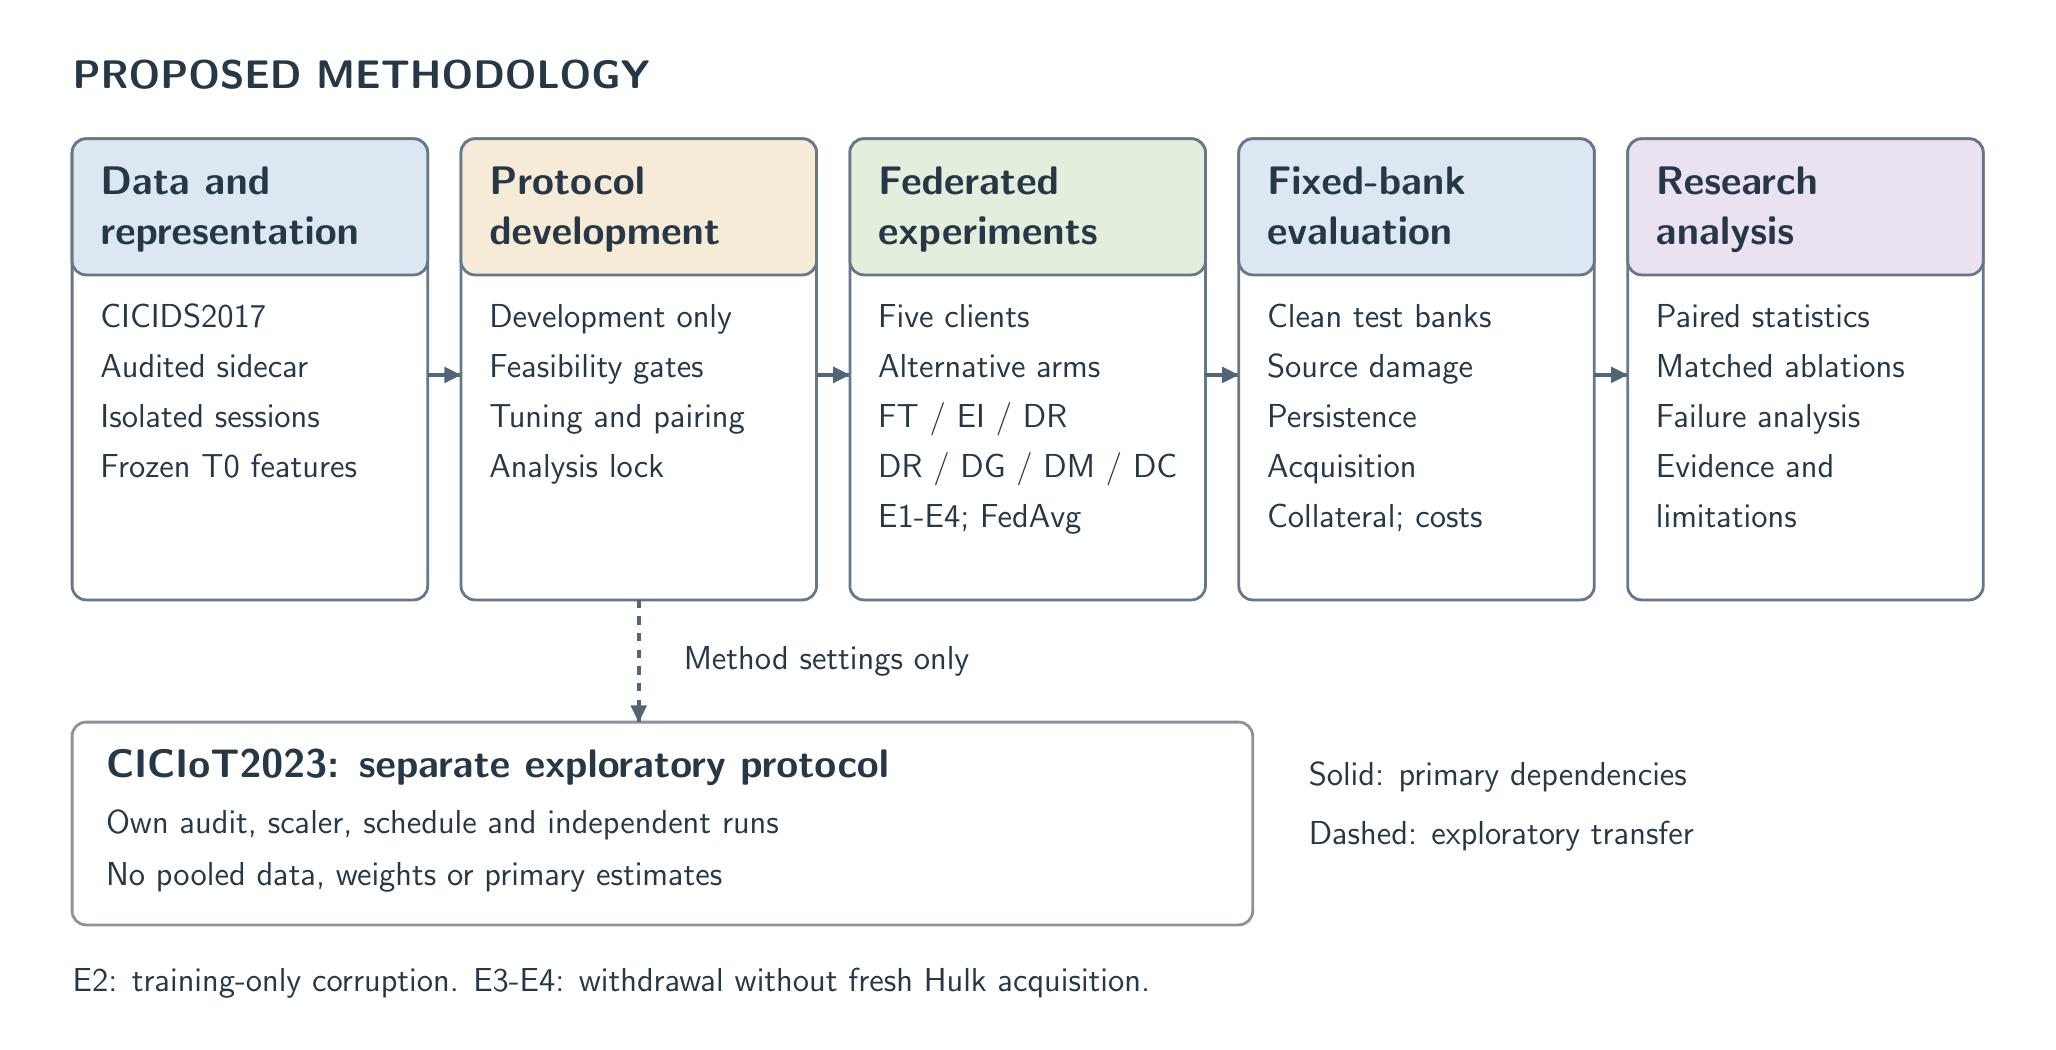
\begin{tikzpicture}[x=1bp,y=-1bp]
\path[use as bounding box] (0,0) rectangle (720,358);
\node[anchor=base west,inner sep=0,text={rgb,255:red,38;green,55;blue,70},font=\sffamily\bfseries\fontsize{15}{17.25}\selectfont] at (16,22) {PROPOSED METHODOLOGY};
\path[draw={rgb,255:red,102;green,119;blue,137},fill={rgb,255:red,255;green,255;blue,255},line width=1bp,rounded corners=5bp] (16,40) rectangle (144,206);
\path[draw={rgb,255:red,102;green,119;blue,137},fill={rgb,255:red,220;green,231;blue,242},line width=1bp,rounded corners=5bp] (16,40) rectangle (144,89);
\node[anchor=base west,inner sep=0,text={rgb,255:red,38;green,55;blue,70},font=\sffamily\bfseries\fontsize{15}{17.25}\selectfont] at (26,60) {Data and};
\node[anchor=base west,inner sep=0,text={rgb,255:red,38;green,55;blue,70},font=\sffamily\bfseries\fontsize{15}{17.25}\selectfont] at (26,78) {representation};
\node[anchor=base west,inner sep=0,text={rgb,255:red,38;green,55;blue,70},font=\sffamily\fontsize{12}{13.799999999999999}\selectfont] at (26,108) {CICIDS2017};
\node[anchor=base west,inner sep=0,text={rgb,255:red,38;green,55;blue,70},font=\sffamily\fontsize{12}{13.799999999999999}\selectfont] at (26,126) {Audited sidecar};
\node[anchor=base west,inner sep=0,text={rgb,255:red,38;green,55;blue,70},font=\sffamily\fontsize{12}{13.799999999999999}\selectfont] at (26,144) {Isolated sessions};
\node[anchor=base west,inner sep=0,text={rgb,255:red,38;green,55;blue,70},font=\sffamily\fontsize{12}{13.799999999999999}\selectfont] at (26,162) {Frozen T0 features};
\path[draw={rgb,255:red,80;green,101;blue,118},line width=1.4bp] (144,125) -- (156,125);
\path[fill={rgb,255:red,80;green,101;blue,118}] (156.000,125.000) -- (150.000,122.000) -- (150.000,128.000) -- cycle;
\path[draw={rgb,255:red,102;green,119;blue,137},fill={rgb,255:red,255;green,255;blue,255},line width=1bp,rounded corners=5bp] (156,40) rectangle (284,206);
\path[draw={rgb,255:red,102;green,119;blue,137},fill={rgb,255:red,245;green,235;blue,215},line width=1bp,rounded corners=5bp] (156,40) rectangle (284,89);
\node[anchor=base west,inner sep=0,text={rgb,255:red,38;green,55;blue,70},font=\sffamily\bfseries\fontsize{15}{17.25}\selectfont] at (166,60) {Protocol};
\node[anchor=base west,inner sep=0,text={rgb,255:red,38;green,55;blue,70},font=\sffamily\bfseries\fontsize{15}{17.25}\selectfont] at (166,78) {development};
\node[anchor=base west,inner sep=0,text={rgb,255:red,38;green,55;blue,70},font=\sffamily\fontsize{12}{13.799999999999999}\selectfont] at (166,108) {Development only};
\node[anchor=base west,inner sep=0,text={rgb,255:red,38;green,55;blue,70},font=\sffamily\fontsize{12}{13.799999999999999}\selectfont] at (166,126) {Feasibility gates};
\node[anchor=base west,inner sep=0,text={rgb,255:red,38;green,55;blue,70},font=\sffamily\fontsize{12}{13.799999999999999}\selectfont] at (166,144) {Tuning and pairing};
\node[anchor=base west,inner sep=0,text={rgb,255:red,38;green,55;blue,70},font=\sffamily\fontsize{12}{13.799999999999999}\selectfont] at (166,162) {Analysis lock};
\path[draw={rgb,255:red,80;green,101;blue,118},line width=1.4bp] (284,125) -- (296,125);
\path[fill={rgb,255:red,80;green,101;blue,118}] (296.000,125.000) -- (290.000,122.000) -- (290.000,128.000) -- cycle;
\path[draw={rgb,255:red,102;green,119;blue,137},fill={rgb,255:red,255;green,255;blue,255},line width=1bp,rounded corners=5bp] (296,40) rectangle (424,206);
\path[draw={rgb,255:red,102;green,119;blue,137},fill={rgb,255:red,228;green,238;blue,221},line width=1bp,rounded corners=5bp] (296,40) rectangle (424,89);
\node[anchor=base west,inner sep=0,text={rgb,255:red,38;green,55;blue,70},font=\sffamily\bfseries\fontsize{15}{17.25}\selectfont] at (306,60) {Federated};
\node[anchor=base west,inner sep=0,text={rgb,255:red,38;green,55;blue,70},font=\sffamily\bfseries\fontsize{15}{17.25}\selectfont] at (306,78) {experiments};
\node[anchor=base west,inner sep=0,text={rgb,255:red,38;green,55;blue,70},font=\sffamily\fontsize{12}{13.799999999999999}\selectfont] at (306,108) {Five clients};
\node[anchor=base west,inner sep=0,text={rgb,255:red,38;green,55;blue,70},font=\sffamily\fontsize{12}{13.799999999999999}\selectfont] at (306,126) {Alternative arms};
\node[anchor=base west,inner sep=0,text={rgb,255:red,38;green,55;blue,70},font=\sffamily\fontsize{12}{13.799999999999999}\selectfont] at (306,144) {FT / EI / DR};
\node[anchor=base west,inner sep=0,text={rgb,255:red,38;green,55;blue,70},font=\sffamily\fontsize{12}{13.799999999999999}\selectfont] at (306,162) {DR / DG / DM / DC};
\node[anchor=base west,inner sep=0,text={rgb,255:red,38;green,55;blue,70},font=\sffamily\fontsize{12}{13.799999999999999}\selectfont] at (306,180) {E1-E4; FedAvg};
\path[draw={rgb,255:red,80;green,101;blue,118},line width=1.4bp] (424,125) -- (436,125);
\path[fill={rgb,255:red,80;green,101;blue,118}] (436.000,125.000) -- (430.000,122.000) -- (430.000,128.000) -- cycle;
\path[draw={rgb,255:red,102;green,119;blue,137},fill={rgb,255:red,255;green,255;blue,255},line width=1bp,rounded corners=5bp] (436,40) rectangle (564,206);
\path[draw={rgb,255:red,102;green,119;blue,137},fill={rgb,255:red,220;green,231;blue,242},line width=1bp,rounded corners=5bp] (436,40) rectangle (564,89);
\node[anchor=base west,inner sep=0,text={rgb,255:red,38;green,55;blue,70},font=\sffamily\bfseries\fontsize{15}{17.25}\selectfont] at (446,60) {Fixed-bank};
\node[anchor=base west,inner sep=0,text={rgb,255:red,38;green,55;blue,70},font=\sffamily\bfseries\fontsize{15}{17.25}\selectfont] at (446,78) {evaluation};
\node[anchor=base west,inner sep=0,text={rgb,255:red,38;green,55;blue,70},font=\sffamily\fontsize{12}{13.799999999999999}\selectfont] at (446,108) {Clean test banks};
\node[anchor=base west,inner sep=0,text={rgb,255:red,38;green,55;blue,70},font=\sffamily\fontsize{12}{13.799999999999999}\selectfont] at (446,126) {Source damage};
\node[anchor=base west,inner sep=0,text={rgb,255:red,38;green,55;blue,70},font=\sffamily\fontsize{12}{13.799999999999999}\selectfont] at (446,144) {Persistence};
\node[anchor=base west,inner sep=0,text={rgb,255:red,38;green,55;blue,70},font=\sffamily\fontsize{12}{13.799999999999999}\selectfont] at (446,162) {Acquisition};
\node[anchor=base west,inner sep=0,text={rgb,255:red,38;green,55;blue,70},font=\sffamily\fontsize{12}{13.799999999999999}\selectfont] at (446,180) {Collateral; costs};
\path[draw={rgb,255:red,80;green,101;blue,118},line width=1.4bp] (564,125) -- (576,125);
\path[fill={rgb,255:red,80;green,101;blue,118}] (576.000,125.000) -- (570.000,122.000) -- (570.000,128.000) -- cycle;
\path[draw={rgb,255:red,102;green,119;blue,137},fill={rgb,255:red,255;green,255;blue,255},line width=1bp,rounded corners=5bp] (576,40) rectangle (704,206);
\path[draw={rgb,255:red,102;green,119;blue,137},fill={rgb,255:red,234;green,226;blue,241},line width=1bp,rounded corners=5bp] (576,40) rectangle (704,89);
\node[anchor=base west,inner sep=0,text={rgb,255:red,38;green,55;blue,70},font=\sffamily\bfseries\fontsize{15}{17.25}\selectfont] at (586,60) {Research};
\node[anchor=base west,inner sep=0,text={rgb,255:red,38;green,55;blue,70},font=\sffamily\bfseries\fontsize{15}{17.25}\selectfont] at (586,78) {analysis};
\node[anchor=base west,inner sep=0,text={rgb,255:red,38;green,55;blue,70},font=\sffamily\fontsize{12}{13.799999999999999}\selectfont] at (586,108) {Paired statistics};
\node[anchor=base west,inner sep=0,text={rgb,255:red,38;green,55;blue,70},font=\sffamily\fontsize{12}{13.799999999999999}\selectfont] at (586,126) {Matched ablations};
\node[anchor=base west,inner sep=0,text={rgb,255:red,38;green,55;blue,70},font=\sffamily\fontsize{12}{13.799999999999999}\selectfont] at (586,144) {Failure analysis};
\node[anchor=base west,inner sep=0,text={rgb,255:red,38;green,55;blue,70},font=\sffamily\fontsize{12}{13.799999999999999}\selectfont] at (586,162) {Evidence and};
\node[anchor=base west,inner sep=0,text={rgb,255:red,38;green,55;blue,70},font=\sffamily\fontsize{12}{13.799999999999999}\selectfont] at (586,180) {limitations};
\path[draw={rgb,255:red,137;green,147;blue,157},fill={rgb,255:red,255;green,255;blue,255},line width=1bp,rounded corners=5bp] (16,250) rectangle (441,323);
\node[anchor=base west,inner sep=0,text={rgb,255:red,38;green,55;blue,70},font=\sffamily\bfseries\fontsize{15}{17.25}\selectfont] at (28,270) {CICIoT2023: separate exploratory protocol};
\node[anchor=base west,inner sep=0,text={rgb,255:red,38;green,55;blue,70},font=\sffamily\fontsize{12}{13.799999999999999}\selectfont] at (28,290) {Own audit, scaler, schedule and independent runs};
\node[anchor=base west,inner sep=0,text={rgb,255:red,38;green,55;blue,70},font=\sffamily\fontsize{12}{13.799999999999999}\selectfont] at (28,309) {No pooled data, weights or primary estimates};
\path[draw={rgb,255:red,80;green,101;blue,118},line width=1.4bp,dashed] (220,206) -- (220,250);
\path[fill={rgb,255:red,80;green,101;blue,118}] (220.000,250.000) -- (223.000,244.000) -- (217.000,244.000) -- cycle;
\node[anchor=base west,inner sep=0,text={rgb,255:red,38;green,55;blue,70},font=\sffamily\fontsize{12}{13.799999999999999}\selectfont] at (236,231) {Method settings only};
\node[anchor=base west,inner sep=0,text={rgb,255:red,38;green,55;blue,70},font=\sffamily\fontsize{12}{13.799999999999999}\selectfont] at (461,273) {Solid: primary dependencies};
\node[anchor=base west,inner sep=0,text={rgb,255:red,38;green,55;blue,70},font=\sffamily\fontsize{12}{13.799999999999999}\selectfont] at (461,294) {Dashed: exploratory transfer};
\node[anchor=base west,inner sep=0,text={rgb,255:red,38;green,55;blue,70},font=\sffamily\fontsize{12}{13.799999999999999}\selectfont] at (16,347) {E2: training-only corruption. E3-E4: withdrawal without fresh Hulk acquisition.};
\end{tikzpicture}
}
\caption{Proposed methodology overview. Solid arrows transfer audited inputs, locked settings, trained checkpoints and predictions/metrics, respectively. Predictions support failure analysis directly. Component experiments receive their own matched evaluations. The dashed branch transfers method settings to a separate exploratory CICIoT2023 protocol; data, weights and primary estimates are not pooled. Exact settings remain in the protocol tables.}
\label{fig:methodology}
\end{figure}

\begin{figure}[htbp]
\centering
\resizebox{\linewidth}{!}{%
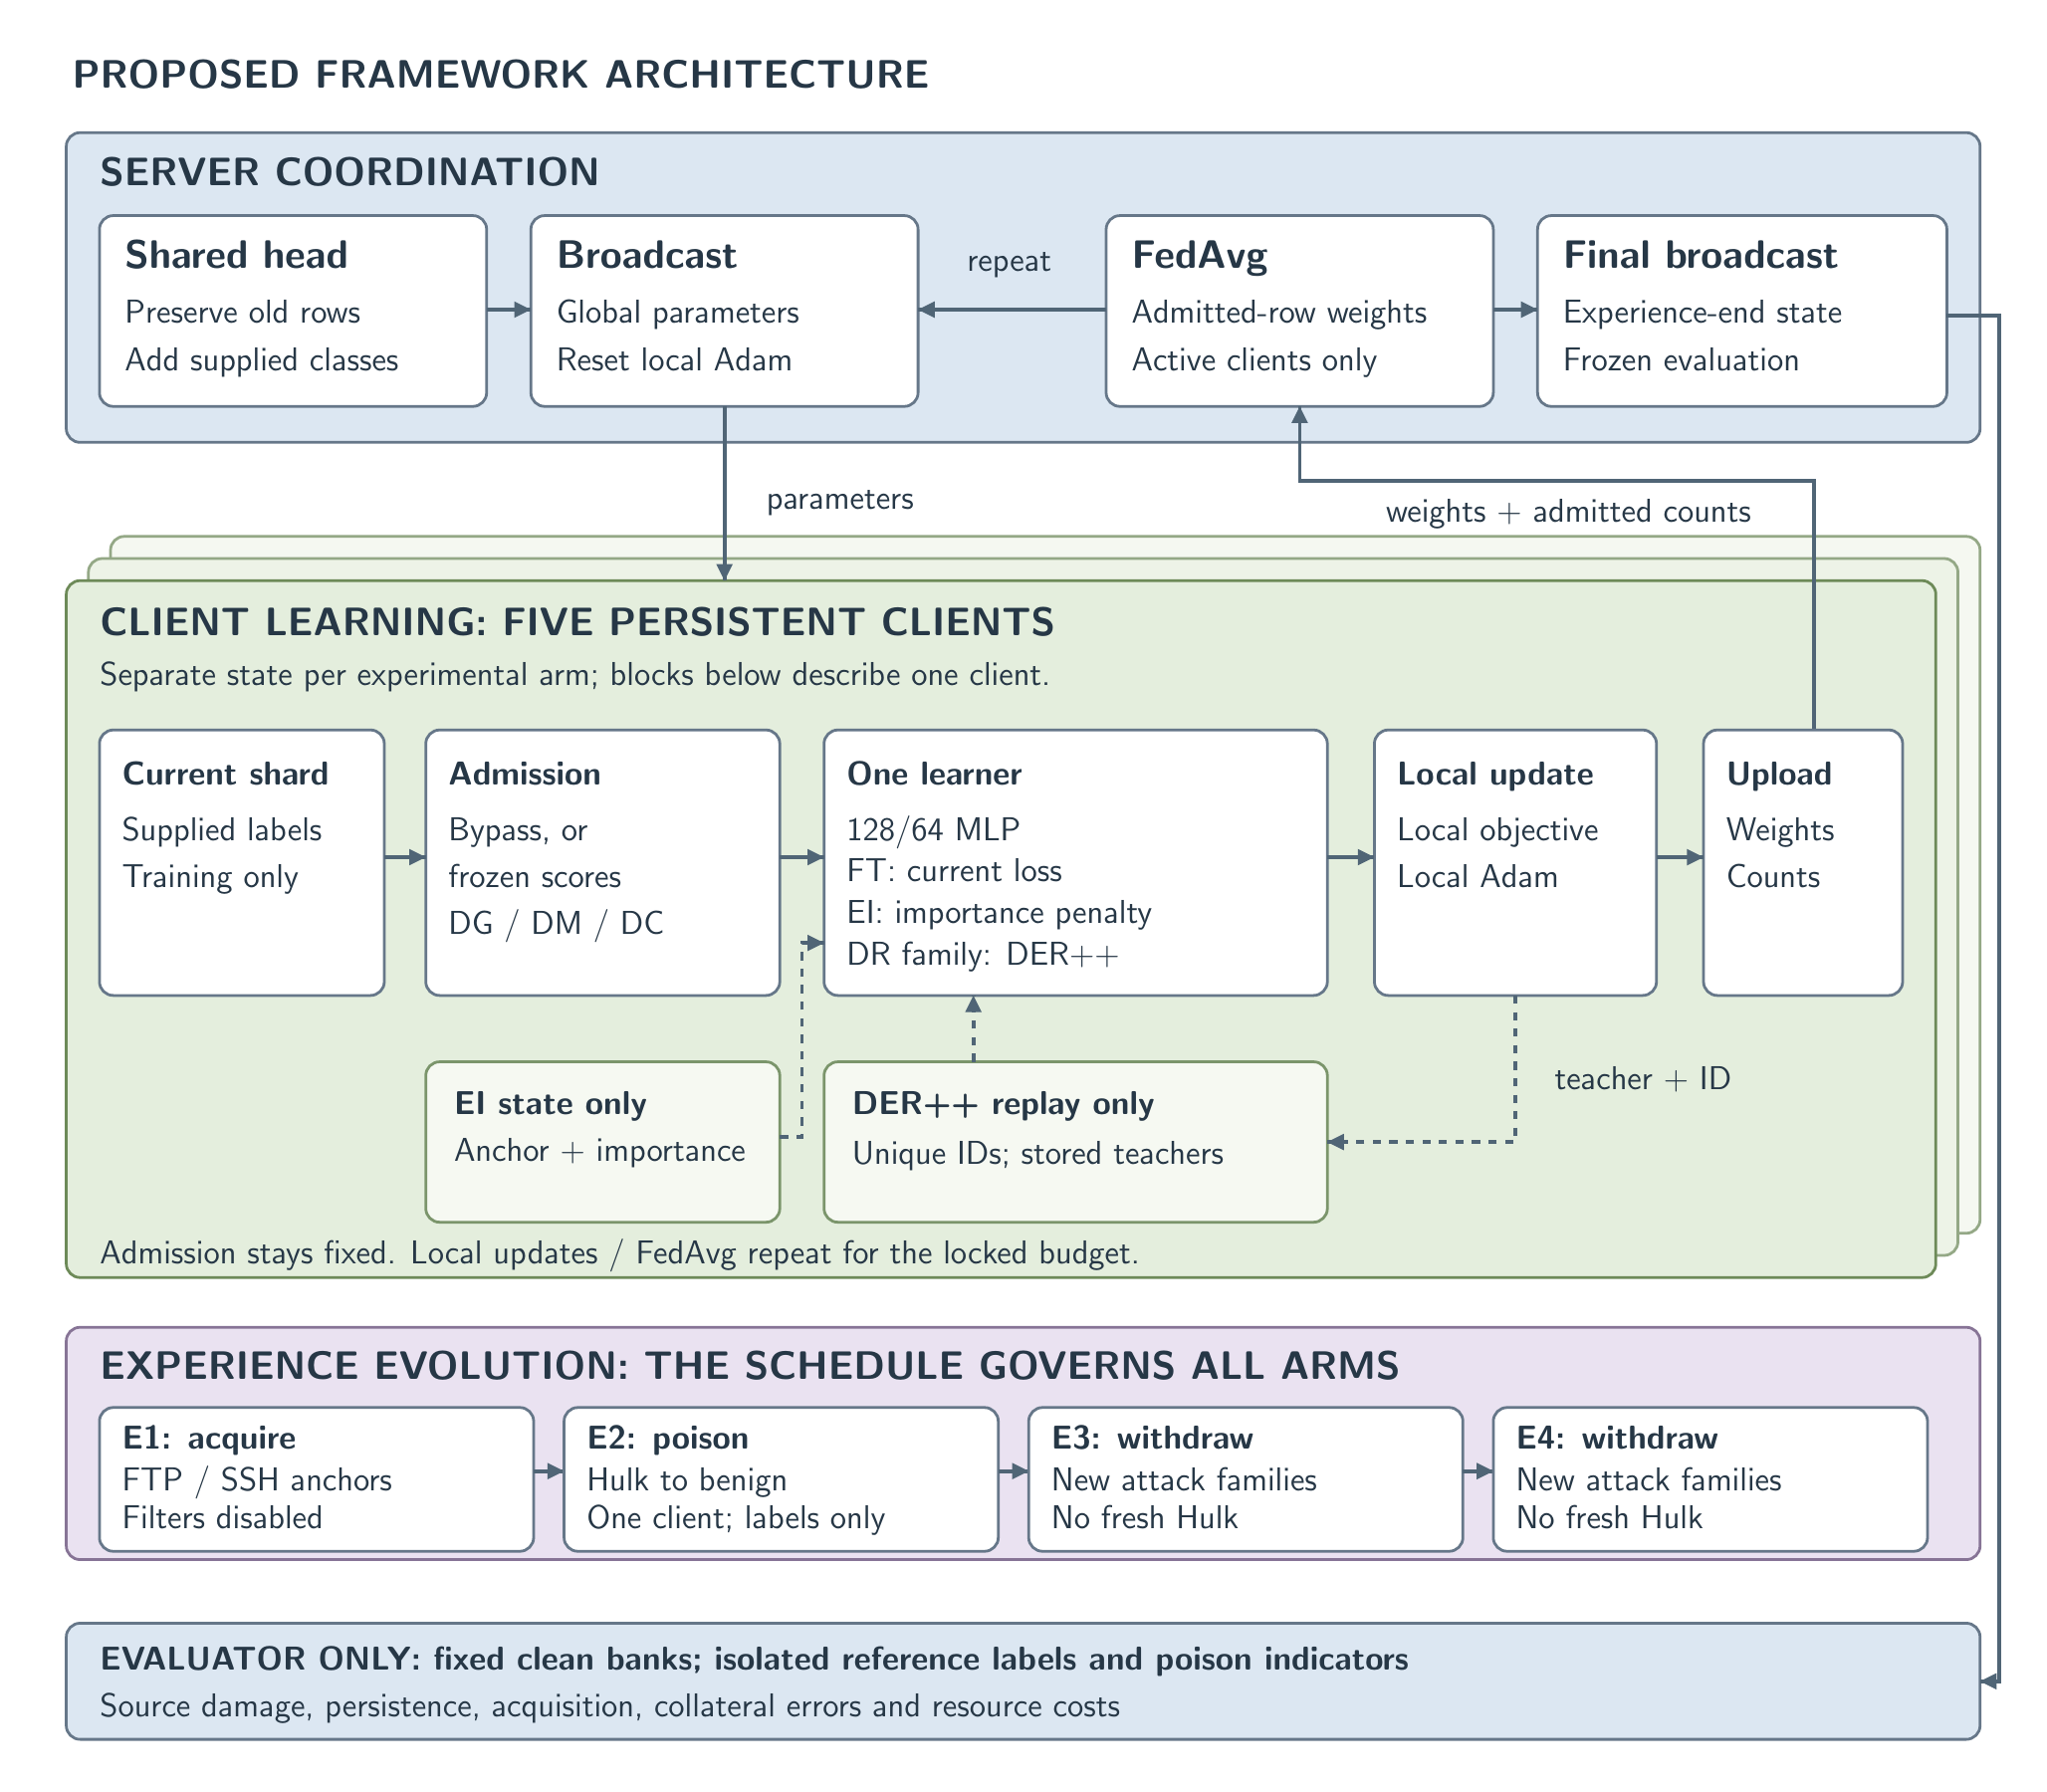
\begin{tikzpicture}[x=1bp,y=-1bp]
\path[use as bounding box] (0,0) rectangle (720,628);
\node[anchor=base west,inner sep=0,text={rgb,255:red,38;green,55;blue,70},font=\sffamily\bfseries\fontsize{15}{17.25}\selectfont] at (16,22) {PROPOSED FRAMEWORK ARCHITECTURE};
\path[draw={rgb,255:red,102;green,119;blue,137},fill={rgb,255:red,220;green,231;blue,242},line width=1bp,rounded corners=5bp] (14,38) rectangle (706,150);
\node[anchor=base west,inner sep=0,text={rgb,255:red,38;green,55;blue,70},font=\sffamily\bfseries\fontsize{15}{17.25}\selectfont] at (26,57) {SERVER COORDINATION};
\path[draw={rgb,255:red,102;green,119;blue,137},fill={rgb,255:red,255;green,255;blue,255},line width=1bp,rounded corners=5bp] (26,68) rectangle (166,137);
\node[anchor=base west,inner sep=0,text={rgb,255:red,38;green,55;blue,70},font=\sffamily\bfseries\fontsize{14}{16.099999999999998}\selectfont] at (35,87) {Shared head};
\node[anchor=base west,inner sep=0,text={rgb,255:red,38;green,55;blue,70},font=\sffamily\fontsize{12}{13.799999999999999}\selectfont] at (35,107) {Preserve old rows};
\node[anchor=base west,inner sep=0,text={rgb,255:red,38;green,55;blue,70},font=\sffamily\fontsize{12}{13.799999999999999}\selectfont] at (35,124) {Add supplied classes};
\path[draw={rgb,255:red,102;green,119;blue,137},fill={rgb,255:red,255;green,255;blue,255},line width=1bp,rounded corners=5bp] (182,68) rectangle (322,137);
\node[anchor=base west,inner sep=0,text={rgb,255:red,38;green,55;blue,70},font=\sffamily\bfseries\fontsize{14}{16.099999999999998}\selectfont] at (191,87) {Broadcast};
\node[anchor=base west,inner sep=0,text={rgb,255:red,38;green,55;blue,70},font=\sffamily\fontsize{12}{13.799999999999999}\selectfont] at (191,107) {Global parameters};
\node[anchor=base west,inner sep=0,text={rgb,255:red,38;green,55;blue,70},font=\sffamily\fontsize{12}{13.799999999999999}\selectfont] at (191,124) {Reset local Adam};
\path[draw={rgb,255:red,102;green,119;blue,137},fill={rgb,255:red,255;green,255;blue,255},line width=1bp,rounded corners=5bp] (390,68) rectangle (530,137);
\node[anchor=base west,inner sep=0,text={rgb,255:red,38;green,55;blue,70},font=\sffamily\bfseries\fontsize{14}{16.099999999999998}\selectfont] at (399,87) {FedAvg};
\node[anchor=base west,inner sep=0,text={rgb,255:red,38;green,55;blue,70},font=\sffamily\fontsize{12}{13.799999999999999}\selectfont] at (399,107) {Admitted-row weights};
\node[anchor=base west,inner sep=0,text={rgb,255:red,38;green,55;blue,70},font=\sffamily\fontsize{12}{13.799999999999999}\selectfont] at (399,124) {Active clients only};
\path[draw={rgb,255:red,102;green,119;blue,137},fill={rgb,255:red,255;green,255;blue,255},line width=1bp,rounded corners=5bp] (546,68) rectangle (694,137);
\node[anchor=base west,inner sep=0,text={rgb,255:red,38;green,55;blue,70},font=\sffamily\bfseries\fontsize{14}{16.099999999999998}\selectfont] at (555,87) {Final broadcast};
\node[anchor=base west,inner sep=0,text={rgb,255:red,38;green,55;blue,70},font=\sffamily\fontsize{12}{13.799999999999999}\selectfont] at (555,107) {Experience-end state};
\node[anchor=base west,inner sep=0,text={rgb,255:red,38;green,55;blue,70},font=\sffamily\fontsize{12}{13.799999999999999}\selectfont] at (555,124) {Frozen evaluation};
\path[draw={rgb,255:red,80;green,101;blue,118},line width=1.4bp] (166,102) -- (182,102);
\path[fill={rgb,255:red,80;green,101;blue,118}] (182.000,102.000) -- (176.000,99.000) -- (176.000,105.000) -- cycle;
\path[draw={rgb,255:red,80;green,101;blue,118},line width=1.4bp] (530,102) -- (546,102);
\path[fill={rgb,255:red,80;green,101;blue,118}] (546.000,102.000) -- (540.000,99.000) -- (540.000,105.000) -- cycle;
\path[draw={rgb,255:red,80;green,101;blue,118},line width=1.4bp] (390,102) -- (322,102);
\path[fill={rgb,255:red,80;green,101;blue,118}] (322.000,102.000) -- (328.000,105.000) -- (328.000,99.000) -- cycle;
\node[anchor=base,inner sep=0,text={rgb,255:red,38;green,55;blue,70},font=\sffamily\fontsize{12}{13.799999999999999}\selectfont] at (355,88) {repeat};
\path[draw={rgb,255:red,148;green,168;blue,134},fill={rgb,255:red,245;green,248;blue,241},line width=1bp,rounded corners=5bp] (30,184) rectangle (706,436);
\path[draw={rgb,255:red,148;green,168;blue,134},fill={rgb,255:red,237;green,243;blue,231},line width=1bp,rounded corners=5bp] (22,192) rectangle (698,444);
\path[draw={rgb,255:red,109;green,138;blue,88},fill={rgb,255:red,228;green,238;blue,221},line width=1bp,rounded corners=5bp] (14,200) rectangle (690,452);
\node[anchor=base west,inner sep=0,text={rgb,255:red,38;green,55;blue,70},font=\sffamily\bfseries\fontsize{15}{17.25}\selectfont] at (26,220) {CLIENT LEARNING: FIVE PERSISTENT CLIENTS};
\node[anchor=base west,inner sep=0,text={rgb,255:red,38;green,55;blue,70},font=\sffamily\fontsize{12}{13.799999999999999}\selectfont] at (26,238) {Separate state per experimental arm; blocks below describe one client.};
\path[draw={rgb,255:red,80;green,101;blue,118},line width=1.4bp] (252,137) -- (252,200);
\path[fill={rgb,255:red,80;green,101;blue,118}] (252.000,200.000) -- (255.000,194.000) -- (249.000,194.000) -- cycle;
\node[anchor=base west,inner sep=0,text={rgb,255:red,38;green,55;blue,70},font=\sffamily\fontsize{12}{13.799999999999999}\selectfont] at (267,174) {parameters};
\path[draw={rgb,255:red,80;green,101;blue,118},line width=1.4bp] (646,254) -- (646,164) -- (460,164) -- (460,137);
\path[fill={rgb,255:red,80;green,101;blue,118}] (460.000,137.000) -- (457.000,143.000) -- (463.000,143.000) -- cycle;
\node[anchor=base west,inner sep=0,text={rgb,255:red,38;green,55;blue,70},font=\sffamily\fontsize{12}{13.799999999999999}\selectfont] at (491,179) {weights + admitted counts};
\path[draw={rgb,255:red,102;green,119;blue,137},fill={rgb,255:red,255;green,255;blue,255},line width=1bp,rounded corners=5bp] (26,254) rectangle (129,350);
\node[anchor=base west,inner sep=0,text={rgb,255:red,38;green,55;blue,70},font=\sffamily\bfseries\fontsize{13}{14.95}\selectfont] at (34,274) {Current shard};
\node[anchor=base west,inner sep=0,text={rgb,255:red,38;green,55;blue,70},font=\sffamily\fontsize{12}{13.799999999999999}\selectfont] at (34,294) {Supplied labels};
\node[anchor=base west,inner sep=0,text={rgb,255:red,38;green,55;blue,70},font=\sffamily\fontsize{12}{13.799999999999999}\selectfont] at (34,311) {Training only};
\path[draw={rgb,255:red,102;green,119;blue,137},fill={rgb,255:red,255;green,255;blue,255},line width=1bp,rounded corners=5bp] (144,254) rectangle (272,350);
\node[anchor=base west,inner sep=0,text={rgb,255:red,38;green,55;blue,70},font=\sffamily\bfseries\fontsize{13}{14.95}\selectfont] at (152,274) {Admission};
\node[anchor=base west,inner sep=0,text={rgb,255:red,38;green,55;blue,70},font=\sffamily\fontsize{12}{13.799999999999999}\selectfont] at (152,294) {Bypass, or};
\node[anchor=base west,inner sep=0,text={rgb,255:red,38;green,55;blue,70},font=\sffamily\fontsize{12}{13.799999999999999}\selectfont] at (152,311) {frozen scores};
\node[anchor=base west,inner sep=0,text={rgb,255:red,38;green,55;blue,70},font=\sffamily\fontsize{12}{13.799999999999999}\selectfont] at (152,328) {DG / DM / DC};
\path[draw={rgb,255:red,102;green,119;blue,137},fill={rgb,255:red,255;green,255;blue,255},line width=1bp,rounded corners=5bp] (288,254) rectangle (470,350);
\node[anchor=base west,inner sep=0,text={rgb,255:red,38;green,55;blue,70},font=\sffamily\bfseries\fontsize{13}{14.95}\selectfont] at (296,274) {One learner};
\node[anchor=base west,inner sep=0,text={rgb,255:red,38;green,55;blue,70},font=\sffamily\fontsize{12}{13.799999999999999}\selectfont] at (296,294) {128/64 MLP};
\node[anchor=base west,inner sep=0,text={rgb,255:red,38;green,55;blue,70},font=\sffamily\fontsize{12}{13.799999999999999}\selectfont] at (296,309) {FT: current loss};
\node[anchor=base west,inner sep=0,text={rgb,255:red,38;green,55;blue,70},font=\sffamily\fontsize{12}{13.799999999999999}\selectfont] at (296,324) {EI: importance penalty};
\node[anchor=base west,inner sep=0,text={rgb,255:red,38;green,55;blue,70},font=\sffamily\fontsize{12}{13.799999999999999}\selectfont] at (296,339) {DR family: DER++};
\path[draw={rgb,255:red,102;green,119;blue,137},fill={rgb,255:red,255;green,255;blue,255},line width=1bp,rounded corners=5bp] (487,254) rectangle (589,350);
\node[anchor=base west,inner sep=0,text={rgb,255:red,38;green,55;blue,70},font=\sffamily\bfseries\fontsize{13}{14.95}\selectfont] at (495,274) {Local update};
\node[anchor=base west,inner sep=0,text={rgb,255:red,38;green,55;blue,70},font=\sffamily\fontsize{12}{13.799999999999999}\selectfont] at (495,294) {Local objective};
\node[anchor=base west,inner sep=0,text={rgb,255:red,38;green,55;blue,70},font=\sffamily\fontsize{12}{13.799999999999999}\selectfont] at (495,311) {Local Adam};
\path[draw={rgb,255:red,102;green,119;blue,137},fill={rgb,255:red,255;green,255;blue,255},line width=1bp,rounded corners=5bp] (606,254) rectangle (678,350);
\node[anchor=base west,inner sep=0,text={rgb,255:red,38;green,55;blue,70},font=\sffamily\bfseries\fontsize{13}{14.95}\selectfont] at (614,274) {Upload};
\node[anchor=base west,inner sep=0,text={rgb,255:red,38;green,55;blue,70},font=\sffamily\fontsize{12}{13.799999999999999}\selectfont] at (614,294) {Weights};
\node[anchor=base west,inner sep=0,text={rgb,255:red,38;green,55;blue,70},font=\sffamily\fontsize{12}{13.799999999999999}\selectfont] at (614,311) {Counts};
\path[draw={rgb,255:red,80;green,101;blue,118},line width=1.4bp] (129,300) -- (144,300);
\path[fill={rgb,255:red,80;green,101;blue,118}] (144.000,300.000) -- (138.000,297.000) -- (138.000,303.000) -- cycle;
\path[draw={rgb,255:red,80;green,101;blue,118},line width=1.4bp] (272,300) -- (288,300);
\path[fill={rgb,255:red,80;green,101;blue,118}] (288.000,300.000) -- (282.000,297.000) -- (282.000,303.000) -- cycle;
\path[draw={rgb,255:red,80;green,101;blue,118},line width=1.4bp] (470,300) -- (487,300);
\path[fill={rgb,255:red,80;green,101;blue,118}] (487.000,300.000) -- (481.000,297.000) -- (481.000,303.000) -- cycle;
\path[draw={rgb,255:red,80;green,101;blue,118},line width=1.4bp] (589,300) -- (606,300);
\path[fill={rgb,255:red,80;green,101;blue,118}] (606.000,300.000) -- (600.000,297.000) -- (600.000,303.000) -- cycle;
\path[draw={rgb,255:red,123;green,149;blue,107},fill={rgb,255:red,246;green,249;blue,242},line width=1bp,rounded corners=5bp] (144,374) rectangle (272,432);
\node[anchor=base west,inner sep=0,text={rgb,255:red,38;green,55;blue,70},font=\sffamily\bfseries\fontsize{13}{14.95}\selectfont] at (154,393) {EI state only};
\node[anchor=base west,inner sep=0,text={rgb,255:red,38;green,55;blue,70},font=\sffamily\fontsize{12}{13.799999999999999}\selectfont] at (154,410) {Anchor + importance};
\path[draw={rgb,255:red,80;green,101;blue,118},line width=1.4bp,dashed] (272,401) -- (280,401) -- (280,331) -- (288,331);
\path[fill={rgb,255:red,80;green,101;blue,118}] (288.000,331.000) -- (282.000,328.000) -- (282.000,334.000) -- cycle;
\path[draw={rgb,255:red,123;green,149;blue,107},fill={rgb,255:red,246;green,249;blue,242},line width=1bp,rounded corners=5bp] (288,374) rectangle (470,432);
\node[anchor=base west,inner sep=0,text={rgb,255:red,38;green,55;blue,70},font=\sffamily\bfseries\fontsize{13}{14.95}\selectfont] at (298,393) {DER++ replay only};
\node[anchor=base west,inner sep=0,text={rgb,255:red,38;green,55;blue,70},font=\sffamily\fontsize{12}{13.799999999999999}\selectfont] at (298,411) {Unique IDs; stored teachers};
\path[draw={rgb,255:red,80;green,101;blue,118},line width=1.4bp,dashed] (342,374) -- (342,350);
\path[fill={rgb,255:red,80;green,101;blue,118}] (342.000,350.000) -- (339.000,356.000) -- (345.000,356.000) -- cycle;
\path[draw={rgb,255:red,80;green,101;blue,118},line width=1.4bp,dashed] (538,350) -- (538,403) -- (470,403);
\path[fill={rgb,255:red,80;green,101;blue,118}] (470.000,403.000) -- (476.000,406.000) -- (476.000,400.000) -- cycle;
\node[anchor=base west,inner sep=0,text={rgb,255:red,38;green,55;blue,70},font=\sffamily\fontsize{12}{13.799999999999999}\selectfont] at (552,384) {teacher + ID};
\node[anchor=base west,inner sep=0,text={rgb,255:red,38;green,55;blue,70},font=\sffamily\fontsize{12}{13.799999999999999}\selectfont] at (26,447) {Admission stays fixed. Local updates / FedAvg repeat for the locked budget.};
\path[draw={rgb,255:red,135;green,116;blue,150},fill={rgb,255:red,234;green,226;blue,241},line width=1bp,rounded corners=5bp] (14,470) rectangle (706,554);
\node[anchor=base west,inner sep=0,text={rgb,255:red,38;green,55;blue,70},font=\sffamily\bfseries\fontsize{15}{17.25}\selectfont] at (26,489) {EXPERIENCE EVOLUTION: THE SCHEDULE GOVERNS ALL ARMS};
\path[draw={rgb,255:red,102;green,119;blue,137},fill={rgb,255:red,255;green,255;blue,255},line width=1bp,rounded corners=5bp] (26,499) rectangle (183,551);
\node[anchor=base west,inner sep=0,text={rgb,255:red,38;green,55;blue,70},font=\sffamily\bfseries\fontsize{13}{14.95}\selectfont] at (34,514) {E1: acquire};
\node[anchor=base west,inner sep=0,text={rgb,255:red,38;green,55;blue,70},font=\sffamily\fontsize{12}{13.799999999999999}\selectfont] at (34,529) {FTP / SSH anchors};
\node[anchor=base west,inner sep=0,text={rgb,255:red,38;green,55;blue,70},font=\sffamily\fontsize{12}{13.799999999999999}\selectfont] at (34,543) {Filters disabled};
\path[draw={rgb,255:red,80;green,101;blue,118},line width=1.4bp] (183,522) -- (194,522);
\path[fill={rgb,255:red,80;green,101;blue,118}] (194.000,522.000) -- (188.000,519.000) -- (188.000,525.000) -- cycle;
\path[draw={rgb,255:red,102;green,119;blue,137},fill={rgb,255:red,255;green,255;blue,255},line width=1bp,rounded corners=5bp] (194,499) rectangle (351,551);
\node[anchor=base west,inner sep=0,text={rgb,255:red,38;green,55;blue,70},font=\sffamily\bfseries\fontsize{13}{14.95}\selectfont] at (202,514) {E2: poison};
\node[anchor=base west,inner sep=0,text={rgb,255:red,38;green,55;blue,70},font=\sffamily\fontsize{12}{13.799999999999999}\selectfont] at (202,529) {Hulk to benign};
\node[anchor=base west,inner sep=0,text={rgb,255:red,38;green,55;blue,70},font=\sffamily\fontsize{12}{13.799999999999999}\selectfont] at (202,543) {One client; labels only};
\path[draw={rgb,255:red,80;green,101;blue,118},line width=1.4bp] (351,522) -- (362,522);
\path[fill={rgb,255:red,80;green,101;blue,118}] (362.000,522.000) -- (356.000,519.000) -- (356.000,525.000) -- cycle;
\path[draw={rgb,255:red,102;green,119;blue,137},fill={rgb,255:red,255;green,255;blue,255},line width=1bp,rounded corners=5bp] (362,499) rectangle (519,551);
\node[anchor=base west,inner sep=0,text={rgb,255:red,38;green,55;blue,70},font=\sffamily\bfseries\fontsize{13}{14.95}\selectfont] at (370,514) {E3: withdraw};
\node[anchor=base west,inner sep=0,text={rgb,255:red,38;green,55;blue,70},font=\sffamily\fontsize{12}{13.799999999999999}\selectfont] at (370,529) {New attack families};
\node[anchor=base west,inner sep=0,text={rgb,255:red,38;green,55;blue,70},font=\sffamily\fontsize{12}{13.799999999999999}\selectfont] at (370,543) {No fresh Hulk};
\path[draw={rgb,255:red,80;green,101;blue,118},line width=1.4bp] (519,522) -- (530,522);
\path[fill={rgb,255:red,80;green,101;blue,118}] (530.000,522.000) -- (524.000,519.000) -- (524.000,525.000) -- cycle;
\path[draw={rgb,255:red,102;green,119;blue,137},fill={rgb,255:red,255;green,255;blue,255},line width=1bp,rounded corners=5bp] (530,499) rectangle (687,551);
\node[anchor=base west,inner sep=0,text={rgb,255:red,38;green,55;blue,70},font=\sffamily\bfseries\fontsize{13}{14.95}\selectfont] at (538,514) {E4: withdraw};
\node[anchor=base west,inner sep=0,text={rgb,255:red,38;green,55;blue,70},font=\sffamily\fontsize{12}{13.799999999999999}\selectfont] at (538,529) {New attack families};
\node[anchor=base west,inner sep=0,text={rgb,255:red,38;green,55;blue,70},font=\sffamily\fontsize{12}{13.799999999999999}\selectfont] at (538,543) {No fresh Hulk};
\path[draw={rgb,255:red,102;green,119;blue,137},fill={rgb,255:red,220;green,231;blue,242},line width=1bp,rounded corners=5bp] (14,577) rectangle (706,619);
\node[anchor=base west,inner sep=0,text={rgb,255:red,38;green,55;blue,70},font=\sffamily\bfseries\fontsize{13}{14.95}\selectfont] at (26,594) {EVALUATOR ONLY: fixed clean banks; isolated reference labels and poison indicators};
\node[anchor=base west,inner sep=0,text={rgb,255:red,38;green,55;blue,70},font=\sffamily\fontsize{12}{13.799999999999999}\selectfont] at (26,611) {Source damage, persistence, acquisition, collateral errors and resource costs};
\path[draw={rgb,255:red,80;green,101;blue,118},line width=1.4bp] (694,104) -- (713,104) -- (713,598) -- (706,598);
\path[fill={rgb,255:red,80;green,101;blue,118}] (706.000,598.000) -- (712.000,601.000) -- (712.000,595.000) -- cycle;
\end{tikzpicture}
}
\caption{Proposed framework architecture. Server coordination and client learning repeat within each experience. FT/EI/DR are alternative learner arms; DG/DM/DC are alternative admission conditions on DER++. EI alone uses importance/anchor state; DER++ arms alone use replay. Dashed client edges denote state access conditional on the selected learner. Final broadcasts update importance/anchor state on eligible clients once per experience. E2 corrupts training labels on one client only; E3/E4 withdraw corruption without fresh Hulk acquisition. The evaluator remains outside admission/inference.}
\label{fig:framework}
\end{figure}

\section{Scope and Validity Threats}
\textbf{Internal validity.} Group reconstruction, reference-label defects, duplicate content and shared optimizer/head policies can confound comparisons. We require the isolation equations, source support and both pilots before final testing. The proposed admission rule can retain low-loss mislabeled source rows.

\textbf{External validity.} Historical captures and simulated ownership cover conditional benchmark shifts. They do not sample independent organizations. CICIoT2023 supplies a separate audited check; CPU timings and update bytes do not measure physical edge energy or network delay.

\textbf{Construct validity.} Source recall, benign-target error, acquisition and anchor scores measure different outcomes. The local agent follows filtering despite corrupt labels; a fully compromised client has wider capability. Teacher and feature versions affect replay semantics.

\textbf{Conclusion validity.} Twelve seeds measure conditional training variability with fixed test banks, excluding capture-sampling uncertainty. Sparse-family intervals require whole-session resampling, not independent-flow binomial assumptions. Signed-rank/permutation interpretation requires symmetry. Ordinary intervals lack simultaneous coverage. Disclose failed runs, exclusions and protocol amendments.

\appendix
\section{Source Verification Record and Folder Mapping}
\label{app:sources}
\begin{table}[htbp]
\centering\footnotesize
\caption{Corpus mapping and verified source locations.}
\label{tab:mapping}
\begin{tabularx}{\linewidth}{L{2.4cm}L{1.0cm}Y}
\toprule
Study & Folder & Verified numerical/section location\\
\midrule
Carillo 2026 & 4 & Table IV: 79.05/68.10/74.49; selected 100-round FedProx setting.\\
Lavaur 2025 & 5 & Section 4.2 clean F1 .966/.945; Section 5.4/Fig. 10 participation dependence; 10,670 runs.\\
Fuhrman 2025 & 6 & Table II: CICIDS2017 AVG/FwdTrans LwF ratios 1.93/2.64; Best-F uses test labels.\\
Sameera 2025 & 7 & Section 5.4.1: clean F1 89.791/94.184\%; abstract improvement ranges are setting-dependent.\\
Cerasuolo 2025 & 8 & Table 7: TON-IoT all/old/new F1 $95.30\pm1.46$/$96.47\pm1.18$/$85.89\pm7.76$\%; PAUC $96.79\pm2.64$\%; 50 exemplars/class, nine packets.\\
Guo 2025 & 9 & Table 6: 83.4/82.1; Table 12: 76.4; Table 5 is applicability.\\
Prasad 2026 & 10 & Table 6: .979596/.979392; additive Section 3.3 versus multiplicative Section 4.7 gate.\\
\bottomrule
\end{tabularx}
\end{table}
The source record distinguishes author manuscripts from versions of record. Carillo's author template year differs from its registered 2026 publication year; the registered date determines corpus eligibility.

The proposed source archive comprises \path{Monday-WorkingHours.pcap_ISCX.csv}, \path{Tuesday-WorkingHours.pcap_ISCX.csv}, \path{Wednesday-workingHours.pcap_ISCX.csv}, \path{Thursday-WorkingHours-Morning-WebAttacks.pcap_ISCX.csv}, \path{Thursday-WorkingHours-Afternoon-Infilteration.pcap_ISCX.csv}, \path{Friday-WorkingHours-Morning.pcap_ISCX.csv}, \path{Friday-WorkingHours-Afternoon-PortScan.pcap_ISCX.csv}, and \path{Friday-WorkingHours-Afternoon-DDos.pcap_ISCX.csv}.
% VERIFY: confirm upstream archive lineage, PCAP/metadata join, timestamp timezone, TCP closure rules and the proposed 120-second session gap.
% VERIFY: confirm corrected-export alignment and final 50/50/50 support counts before freezing scored families.

\begin{thebibliography}{99}
\bibitem{phase1} Saneedullah and A. Bilal, ``Continual learning for network security,'' frozen Computer Networks Phase 1 course report, 2026.
\bibitem{ge} J. Ge, Y. Feng, and K. Sakurai, ``A stage-wise framework using class-incremental learning for unknown DoS attack detection,'' \emph{Future Internet}, vol. 18, no. 3, Art. 145, 2026. \url{https://doi.org/10.3390/fi18030145}.
\bibitem{wu} Z. Wu, B. He, Z. Si, C. Qiu, X. Liao, and C. Su, ``Communication-efficient federated class-incremental intrusion detection for edge IoT networks,'' \emph{Sensors}, vol. 26, no. 14, Art. 4630, 2026. \url{https://doi.org/10.3390/s26144630}.
\bibitem{luo} F. Luo, S. Fan, X. Li, and W. Xu, ``Adaptive feature distillation-based continuous authentication against RF fingerprint drift for power equipment,'' \emph{Future Internet}, vol. 18, no. 9, Art. 457, 2026. \url{https://doi.org/10.3390/fi18090457}.
\bibitem{clarivate} Clarivate, ``Clarivate unveils the 2025 Journal Citation Reports,'' Jun. 18, 2025. \url{https://clarivate.com/news/clarivate-unveils-the-2025-journal-citation-reports/}. This announcement verifies the edition, not individual category quartiles.
\bibitem{carillo} R. Carillo, F. Cerasuolo, G. Bovenzi, D. Ciuonzo, and A. Pescap\`e, ``A federated and incremental network intrusion detection system for IoT emerging threats,'' \emph{IEEE Trans. Network and Service Management}, vol. 23, pp. 3865--3880, 2026. \url{https://doi.org/10.1109/TNSM.2026.3675031}. Free author PDF: \url{https://domenicociuonzo.wordpress.com/wp-content/uploads/2026/03/early_access_tnsm26_fedcil_ids.pdf}.
\bibitem{lavaur} L. Lavaur, Y. Busnel, and F. Autrel, ``Investigating the impact of label-flipping attacks against federated learning for collaborative intrusion detection,'' \emph{Computers \& Security}, vol. 156, Art. 104462, 2025. \url{https://doi.org/10.1016/j.cose.2025.104462}. Free PDF: \url{https://orbilu.uni.lu/bitstream/10993/65906/1/Investigating_the_Impact_of_Label_flipping_Attacks_against_Federated_Learning_for_Collaborative_Intrusion_Detection.pdf}.
\bibitem{cnd} S. Fuhrman, O. Gungor, and T. Rosing, ``CND-IDS: Continual novelty detection for intrusion detection systems,'' in \emph{Proc. ACM/IEEE DAC}, 2025, pp. 1--7. \url{https://doi.org/10.1109/DAC63849.2025.11132541}. Free author PDF: \url{https://arxiv.org/pdf/2502.14094}.
\bibitem{wei} Sameera K. M., Vinod P., A. Rocha, Rafidha Rehiman K. A., and M. Conti, ``WeiDetect: Weibull distribution-based defense against poisoning attacks in federated learning for network intrusion detection systems,'' \emph{J. Information Security and Applications}, vol. 95, Art. 104275, 2025. \url{https://doi.org/10.1016/j.jisa.2025.104275}. Free author PDF: \url{https://arxiv.org/pdf/2504.04367v2}.
\bibitem{cerasuolo} F. Cerasuolo, G. Bovenzi, D. Ciuonzo, and A. Pescap\`e, ``Attack-adaptive network intrusion detection systems for IoT networks through class incremental learning,'' \emph{Computer Networks}, vol. 263, Art. 111228, 2025. \url{https://doi.org/10.1016/j.comnet.2025.111228}. Free author PDF: \url{https://domenicociuonzo.wordpress.com/wp-content/uploads/2025/03/comnet25_cil_ids.pdf}.
\bibitem{guo} C. Guo, X. Li, J. Cheng, S. Yang, and H. Gong, ``Continual learning for intrusion detection under evolving network threats,'' \emph{Future Internet}, vol. 17, no. 10, Art. 456, 2025. \url{https://doi.org/10.3390/fi17100456}. Free PDF: \url{https://mdpi-res.com/d_attachment/futureinternet/futureinternet-17-00456/article_deploy/futureinternet-17-00456.pdf}.
\bibitem{ensemble} A. Prasad, I. Aljubayri, M. Z. Khan, and A. Noorwali, ``Resilient federated ensemble learning for IoT intrusion detection in adversarial and imbalanced environments,'' \emph{Computer Modeling in Engineering \& Sciences}, vol. 147, no. 3, Art. 48, 2026. \url{https://doi.org/10.32604/cmes.2026.082021}. Free PDF: \url{https://cdn.techscience.cn/files/CMES/2026/TSP_CMES-147-3/TSP_CMES_82021/TSP_CMES_82021.pdf}.
\bibitem{coteach} B. Han et al., ``Co-teaching: Robust training of deep neural networks with extremely noisy labels,'' in \emph{Advances in Neural Information Processing Systems}, vol. 31, 2018. \url{https://arxiv.org/abs/1804.06872}.
% VERIFY: optional proceedings page range for Han et al.; existence/title/authors/year verified.
\bibitem{mentornet} L. Jiang, Z. Zhou, T. Leung, L.-J. Li, and L. Fei-Fei, ``MentorNet: Learning data-driven curriculum for very deep neural networks on corrupted labels,'' in \emph{Proc. ICML}, PMLR, vol. 80, pp. 2304--2313, 2018. \url{https://proceedings.mlr.press/v80/jiang18c.html}.
\bibitem{fedavg} B. McMahan, E. Moore, D. Ramage, S. Hampson, and B. Ag\"uera y Arcas, ``Communication-efficient learning of deep networks from decentralized data,'' in \emph{Proc. AISTATS}, PMLR, vol. 54, pp. 1273--1282, 2017. \url{https://proceedings.mlr.press/v54/mcmahan17a.html}.
\bibitem{ewc} J. Kirkpatrick et al., ``Overcoming catastrophic forgetting in neural networks,'' \emph{Proc. National Academy of Sciences}, vol. 114, no. 13, pp. 3521--3526, 2017. \url{https://doi.org/10.1073/pnas.1611835114}.
\bibitem{lwf} Z. Li and D. Hoiem, ``Learning without forgetting,'' \emph{IEEE Trans. Pattern Analysis and Machine Intelligence}, vol. 40, no. 12, pp. 2935--2947, 2018. \url{https://doi.org/10.1109/TPAMI.2017.2773081}.
\bibitem{tiny} A. Chaudhry et al., ``On tiny episodic memories in continual learning,'' arXiv:1902.10486, 2019. \url{https://arxiv.org/abs/1902.10486}.
\bibitem{der} P. Buzzega, M. Boschini, A. Porrello, D. Abati, and S. Calderara, ``Dark experience for general continual learning: A strong, simple baseline,'' in \emph{Advances in Neural Information Processing Systems}, vol. 33, pp. 15920--15930, 2020. \url{https://arxiv.org/abs/2004.07211}.
\bibitem{adam} D. P. Kingma and J. Ba, ``Adam: A method for stochastic optimization,'' in \emph{Proc. ICLR}, 2015. \url{https://arxiv.org/abs/1412.6980}.
\bibitem{vitter} J. S. Vitter, ``Random sampling with a reservoir,'' \emph{ACM Trans. Mathematical Software}, vol. 11, no. 1, pp. 37--57, 1985. \url{https://doi.org/10.1145/3147.3165}.
\bibitem{hsu} T.-M. H. Hsu, H. Qi, and M. Brown, ``Measuring the effects of non-identical data distribution for federated visual classification,'' arXiv:1909.06335, 2019. \url{https://arxiv.org/abs/1909.06335}.
\bibitem{tolpegin} V. Tolpegin, S. Truex, M. E. Gursoy, and L. Liu, ``Data poisoning attacks against federated learning systems,'' in \emph{Proc. ESORICS}, 2020. \url{https://arxiv.org/abs/2007.08432}.
% VERIFY: ESORICS volume/page range for Tolpegin et al.; title/authors/year verified.
\bibitem{krum} P. Blanchard, E. M. El Mhamdi, R. Guerraoui, and J. Stainer, ``Machine learning with adversaries: Byzantine tolerant gradient descent,'' in \emph{Advances in Neural Information Processing Systems}, vol. 30, 2017. \url{https://proceedings.neurips.cc/paper_files/paper/2017/file/f4b9ec30ad9f68f89b29639786cb62ef-Paper.pdf}.
% VERIFY: optional proceedings page range for Blanchard et al.; title/authors/year verified.
\bibitem{yin} D. Yin, Y. Chen, R. Kannan, and P. Bartlett, ``Byzantine-robust distributed learning,'' in \emph{Proc. ICML}, PMLR, vol. 80, pp. 5650--5659, 2018. \url{https://proceedings.mlr.press/v80/yin18a.html}.
\bibitem{dataset} I. Sharafaldin, A. H. Lashkari, and A. A. Ghorbani, ``Toward generating a new intrusion detection dataset and intrusion traffic characterization,'' in \emph{Proc. ICISSP}, 2018, pp. 108--116. \url{https://doi.org/10.5220/0006639801080116}.
\bibitem{iot} Canadian Institute for Cybersecurity, ``CIC IoT Dataset 2023,'' University of New Brunswick, 2023. \url{https://www.unb.ca/cic/datasets/iotdataset-2023.html}.
\bibitem{engelen} G. Engelen, V. Rimmer, and W. Joosen, ``Troubleshooting an intrusion detection dataset: The CICIDS2017 case study,'' in \emph{Proc. IEEE Security and Privacy Workshops}, 2021, pp. 7--12. \url{https://doi.org/10.1109/SPW53761.2021.00009}.
\bibitem{gem} D. Lopez-Paz and M. Ranzato, ``Gradient episodic memory for continual learning,'' in \emph{Advances in Neural Information Processing Systems}, vol. 30, 2017. \url{https://arxiv.org/abs/1706.08840}.
% VERIFY: optional proceedings page range for Lopez-Paz and Ranzato; title/authors/year verified.
\bibitem{clmetrics} N. D\'iaz-Rodr\'iguez, V. Lomonaco, D. Filliat, and D. Maltoni, ``Don't forget, there is more than forgetting: New metrics for continual learning,'' arXiv:1810.13166, 2018. \url{https://arxiv.org/abs/1810.13166}.
\bibitem{wilcoxon} F. Wilcoxon, ``Individual comparisons by ranking methods,'' \emph{Biometrics Bulletin}, vol. 1, no. 6, pp. 80--83, 1945. \url{https://doi.org/10.2307/3001968}.
\bibitem{holm} S. Holm, ``A simple sequentially rejective multiple test procedure,'' \emph{Scandinavian Journal of Statistics}, vol. 6, no. 2, pp. 65--70, 1979.
\end{thebibliography}
\end{document}
